%% (Master) Thesis template
% Template version used: v1.4
%
% Largely adapted from Adrian Nievergelt's template for the ADPS
% (lecture notes) project.


%% We use the memoir class because it offers a many easy to use features.
\documentclass[11pt,a4paper,titlepage]{memoir}

%% Packages
%% ========

%% LaTeX Font encoding -- DO NOT CHANGE
\usepackage[OT1]{fontenc}

%% Babel provides support for languages.  'english' uses British
%% English hyphenation and text snippets like "Figure" and
%% "Theorem". Use the option 'ngerman' if your document is in German.
%% Use 'american' for American English.  Note that if you change this,
%% the next LaTeX run may show spurious errors.  Simply run it again.
%% If they persist, remove the .aux file and try again.
\usepackage[ngerman, english]{babel}

%% Input encoding 'utf8'. In some cases you might need 'utf8x' for
%% extra symbols. Not all editors, especially on Windows, are UTF-8
%% capable, so you may want to use 'latin1' instead.
\usepackage[utf8]{inputenc}

%% This changes default fonts for both text and math mode to use Herman Zapfs
%% excellent Palatino font.  Do not change this.
\usepackage[sc]{mathpazo}

%% The AMS-LaTeX extensions for mathematical typesetting.  Do not
%% remove.
\usepackage{amsmath,amssymb,amsfonts,mathrsfs}

%% NTheorem is a reimplementation of the AMS Theorem package. This
%% will allow us to typeset theorems like examples, proofs and
%% similar.  Do not remove.
%% NOTE: Must be loaded AFTER amsmath, or the \qed placement will
%% break
\usepackage[amsmath,thmmarks]{ntheorem}

%% LaTeX' own graphics handling
\usepackage{graphicx}

%% We unfortunately need this for the Rules chapter.  Remove it
%% afterwards; or at least NEVER use its underlining features.
\usepackage{soul}

%% This allows you to add .pdf files. It is used to add the
%% declaration of originality.
\usepackage{pdfpages}

%% Some more packages that you may want to use.  Have a look at the
%% file, and consult the package docs for each.
%% See the TeXed file for more explanations

%% [OPT] Multi-rowed cells in tabulars
%\usepackage{multirow}

%% [REC] Intelligent cross reference package. This allows for nice
%% combined references that include the reference and a hint to where
%% to look for it.
\usepackage{varioref}

%% [OPT] Easily changeable quotes with \enquote{Text}
%\usepackage[german=swiss]{csquotes}

%% [REC] Format dates and time depending on locale
\usepackage{datetime}

%% [OPT] Provides a \cancel{} command to stroke through mathematics.
%\usepackage{cancel}

%% [NEED] This allows for additional typesetting tools in mathmode.
%% See its excellent documentation.
\usepackage{mathtools}

%% [ADV] Conditional commands
%\usepackage{ifthen}

%% [OPT] Manual large braces or other delimiters.
%\usepackage{bigdelim, bigstrut}

%% [REC] Alternate vector arrows. Use the command \vv{} to get scaled
%% vector arrows.
\usepackage[h]{esvect}

%% [NEED] Some extensions to tabulars and array environments.
\usepackage{array}

%% [OPT] Postscript support via pstricks graphics package. Very
%% diverse applications.
%\usepackage{pstricks,pst-all}

%% [?] This seems to allow us to define some additional counters.
%\usepackage{etex}

%% [ADV] XY-Pic to typeset some matrix-style graphics
%\usepackage[all]{xy}

%% [OPT] This is needed to generate an index at the end of the
%% document.
%\usepackage{makeidx}

%% [OPT] Fancy package for source code listings.  The template text
%% needs it for some LaTeX snippets; remove/adapt the \lstset when you
%% remove the template content.
\usepackage{listings}
\lstset{
    %language=C++, % We have multiple languages in our thesis
    basicstyle={\normalfont\ttfamily},
    frame=tb,
    framexleftmargin=1.75em,
    xleftmargin=1.75em,
    %xrightmargin=0.25em,
    numbers=left,
    stepnumber=1,
    showstringspaces=false,
    breaklines=true
}

\lstdefinestyle{C++}{
    language=C++,
    keywordstyle=\color{blue},
    stringstyle=\color{red},
    commentstyle=\color{green},
    morecomment=[l][\color{magenta}]{\#}
}

%% [REC] Fancy character protrusion.  Must be loaded after all fonts.
\usepackage{microtype}

%% [REC] Nicer tables.  Read the excellent documentation.
\usepackage{booktabs}

%% \usepackage[a4paper]{geometry}
%% \usepackage{caption}
 \usepackage{subcaption}
%% \usepackage{xcolor}

%% Uncomment for floatbarrier in sections
%\usepackage[section]{placeins}

%% Plots
\usepackage{pgfplots}
%\pgfplotsset{compat=1.8}
%\usepgfplotslibrary{statistics}

%% Filetree
\usepackage{dirtree}

%% Draw diagram
\usetikzlibrary{arrows,positioning,shapes}

%% Disable word-break
%\usepackage[none]{hyphenat}
\hyphenpenalty 10000

%% List spacing
\usepackage{enumitem}
\setlist{nosep}
%\setlist{noitemsep}

%% Our layout configuration.  DO NOT CHANGE.
%% Memoir layout setup

%% NOTE: You are strongly advised not to change any of them unless you
%% know what you are doing.  These settings strongly interact in the
%% final look of the document.

% Dependencies
\usepackage{layout/logo}

% Turn extra space before chapter headings off.
\setlength{\beforechapskip}{0pt}

\nonzeroparskip
\parindent=0pt
\defaultlists

% Chapter style redefinition
\makeatletter

\if@twoside
  \pagestyle{Ruled}
  \copypagestyle{chapter}{Ruled}
\else
  \pagestyle{ruled}
  \copypagestyle{chapter}{ruled}
\fi
\makeoddhead{chapter}{}{}{}
\makeevenhead{chapter}{}{}{}
\makeheadrule{chapter}{\textwidth}{0pt}
\copypagestyle{abstract}{empty}

\makechapterstyle{bianchimod}{%
  \chapterstyle{default}
  \renewcommand*{\chapnamefont}{\normalfont\Large\sffamily}
  \renewcommand*{\chapnumfont}{\normalfont\Large\sffamily}
  \renewcommand*{\printchaptername}{%
    \chapnamefont\centering\@chapapp}
  \renewcommand*{\printchapternum}{\chapnumfont {\thechapter}}
  \renewcommand*{\chaptitlefont}{\normalfont\huge\sffamily}
  \renewcommand*{\printchaptertitle}[1]{%
    \hrule\vskip\onelineskip \centering \chaptitlefont\textbf{\vphantom{gyM}##1}\par}
  \renewcommand*{\afterchaptertitle}{\vskip\onelineskip \hrule\vskip
    \afterchapskip}
  \renewcommand*{\printchapternonum}{%
    \vphantom{\chapnumfont {9}}\afterchapternum}}

% Use the newly defined style
\chapterstyle{bianchimod}

\setsecheadstyle{\Large\bfseries\sffamily}
\setsubsecheadstyle{\large\bfseries\sffamily}
\setsubsubsecheadstyle{\bfseries\sffamily}
\setparaheadstyle{\normalsize\bfseries\sffamily}
\setsubparaheadstyle{\normalsize\itshape\sffamily}
\setsubparaindent{0pt}

% Set captions to a more separated style for clearness
\captionnamefont{\sffamily\bfseries\footnotesize}
\captiontitlefont{\sffamily\footnotesize}
\setlength{\intextsep}{16pt}
\setlength{\belowcaptionskip}{1pt}

% Set section and TOC numbering depth to subsection
\setsecnumdepth{subsubsection}
\settocdepth{subsubsection}

%% Titlepage adjustments
\pretitle{\vspace{0pt plus 0.7fill}\begin{center}\HUGE\sffamily\bfseries}
\posttitle{\end{center}\par}
\preauthor{\par\begin{center}\let\and\\\Large\sffamily}
\postauthor{\end{center}}
\predate{\par\begin{center}\Large\sffamily}
\postdate{\end{center}}

\def\@advisors{}
\newcommand{\advisors}[1]{\def\@advisors{#1}}
\def\@department{}
\newcommand{\department}[1]{\def\@department{#1}}
\def\@thesistype{}
\newcommand{\thesistype}[1]{\def\@thesistype{#1}}

\renewcommand{\maketitlehooka}{\noindent\logo[2in]}

\renewcommand{\maketitlehookb}{\vspace{1in}%
  \par\begin{center}\Large\sffamily\@thesistype\end{center}}

\renewcommand{\maketitlehookd}{%
  \vfill\par
  \begin{flushright}
    \sffamily
    \@advisors\par
    \@department NKSA G19E
  \end{flushright}
}

\checkandfixthelayout

\setlength{\droptitle}{-48pt}

\makeatother

% This defines how theorems should look. Best leave as is.
\theoremstyle{plain}
\setlength\theorempostskipamount{0pt}

%%% Local Variables:
%%% mode: latex
%%% TeX-master: "thesis"
%%% End:


%% Theorem environments.  You will have to adapt this for a German
%% thesis.
%% Theorem-like environments

%% This can be changed according to language. You can comment out the ones you
%% don't need.

\numberwithin{equation}{chapter}

%% German theorems
%\newtheorem{satz}{Satz}[chapter]
%\newtheorem{beispiel}[satz]{Beispiel}
%\newtheorem{bemerkung}[satz]{Bemerkung}
%\newtheorem{korrolar}[satz]{Korrolar}
%\newtheorem{definition}[satz]{Definition}
%\newtheorem{lemma}[satz]{Lemma}
%\newtheorem{proposition}[satz]{Proposition}

%% English variants
\newtheorem{theorem}{Theorem}[chapter]
\newtheorem{example}[theorem]{Example}
\newtheorem{remark}[theorem]{Remark}
\newtheorem{corollary}[theorem]{Corollary}
\newtheorem{definition}[theorem]{Definition}
\newtheorem{lemma}[theorem]{Lemma}
\newtheorem{proposition}[theorem]{Proposition}

%% Proof environment with a small square as a "qed" symbol
\theoremstyle{nonumberplain}
\theorembodyfont{\normalfont}
\theoremsymbol{\ensuremath{\square}}
\newtheorem{proof}{Proof}
%\newtheorem{beweis}{Beweis}


%% Helpful macros.
%% Custom commands
%% ===============

%% Special characters for number sets, e.g. real or complex numbers.
\newcommand{\C}{\mathbb{C}}
\newcommand{\K}{\mathbb{K}}
\newcommand{\N}{\mathbb{N}}
\newcommand{\Q}{\mathbb{Q}}
\newcommand{\R}{\mathbb{R}}
\newcommand{\Z}{\mathbb{Z}}
\newcommand{\X}{\mathbb{X}}

%% Fixed/scaling delimiter examples (see mathtools documentation)
\DeclarePairedDelimiter\abs{\lvert}{\rvert}
\DeclarePairedDelimiter\norm{\lVert}{\rVert}

%% Use the alternative epsilon per default and define the old one as \oldepsilon
\let\oldepsilon\epsilon
\renewcommand{\epsilon}{\ensuremath\varepsilon}

%% Also set the alternate phi as default.
\let\oldphi\phi
\renewcommand{\phi}{\ensuremath{\varphi}}

%% Highlight single codeword
\newcommand{\codeword}[1]{
    \textcolor{blue}{\lstinline[xleftmargin=5.5em]{#1}}
}

%% Make document internal hyperlinks wherever possible. (TOC, references)
%% This MUST be loaded after varioref, which is loaded in 'extrapackages'
%% above.  We just load it last to be safe.
\usepackage[linkcolor=black,colorlinks=true,citecolor=black,filecolor=black]{hyperref}


% Our packages
% Biblatex for a better bibliography
\usepackage{hyphenat}
\usepackage{array}
\usepackage{caption}
\usepackage{subcaption}
\usepackage{makecell}
% \usepackage[citestyle=numeric, bibstyle=numeric, sorting=none]{biblatex}
\usepackage[backend=biber, style=apa, 
natbib=true]{biblatex}
\usepackage{cleveref}
\usepackage[babel, german=quotes]{csquotes}
\usepackage{listings}
\usepackage{datetime}
\newcommand{\code}[1]{\texttt{#1}}
\lstset{extendedchars=\true}
\lstset{inputencoding=utf8}
\addbibresource{refs.bib}

% Our configs
\emergencystretch=\maxdimen
% \DeclareLabeldate{
%   \field{date}
%   \field{event}
%   \field{orig}
%   \field{url}
%   \literal{nodate}
% }

\renewcommand\cite{\citep}

\selectlanguage{ngerman}
\newdateformat{dateFormat}{\THEDAY{. }\monthnamengerman[\THEMONTH], \THEYEAR}
%% Document information
%% ====================

\title{MensaRating WebApp}
\author{Ian Wasser, Robin Steiner, Nicolas Kaufmann, Valentin Gisi}
\thesistype{EINF Projekt: Milestone II}
\advisors{Betreut durch: Martina Vàzquez}
\date{\dateFormat\today}

\begin{document}

\newcommand*{\doubleref}[1]{\hyperref[{#1}]{\ref*{#1} \nameref*{#1}}}
%https://tex.stackexchange.com/questions/121865/nameref-how-to-display-section-name-and-its-number

\frontmatter

%% Title page is autogenerated from document information above.  DO
%% NOT CHANGE.
\begin{titlingpage}
  \calccentering{\unitlength}
  \begin{adjustwidth*}{\unitlength-24pt}{-\unitlength-24pt}
    \maketitle
  \end{adjustwidth*}
\end{titlingpage}

%% The abstract of your thesis.  Edit the file as needed.
\selectlanguage{english}
% \input{chapters/abstract}
\selectlanguage{ngerman}

%% TOC with the proper setup, do not change.
\cleartorecto
\begin{KeepFromToc}
\tableofcontents
\end{KeepFromToc}
\mainmatter

%% Template content
%% Some commands used in this file
\newcommand{\package}{\emph}

\chapter{Introduction}

This is version \verb-v1.4- of the template.

We assume that you found this template on our institute's website, so
we do not repeat everything stated there.  Consult the website again
for pointers to further reading about \LaTeX{}.  This chapter only
gives a brief overview of the files you are looking at.

\section{Features}
\label{sec:features}

The rest of this document shows off a few features of the template
files.  Look at the source code to see which macros we used!

The template is divided into \TeX{} files as follows:
\begin{enumerate}
\item \texttt{thesis.tex} is the main file.
\item \texttt{extrapackages.tex} holds extra package includes.
\item \texttt{layoutsetup.tex} defines the style used in this document.
\item \texttt{theoremsetup.tex} declares the theorem-like environments.
\item \texttt{macrosetup.tex} defines extra macros that you may find
  useful.
\item \texttt{introduction.tex} contains this text.
\item \texttt{sections.tex} is a quick demo of each sectioning level
  available.
\item \texttt{refs.bib} is an example bibliography file.  You can use
  Bib\TeX{} to quote references.  For example, read
  \cite{bringhurst1996ets} if you can get a hold of it.
\end{enumerate}


\subsection{Extra package includes}

The file \texttt{extrapackages.tex} lists some packages that usually
come in handy.  Simply have a look at the source code.  We have
added the following comments based on our experiences:
\begin{description}
\item[REC] This package is recommended.
\item[OPT] This package is optional.  It usually solves a specific
  problem in a clever way.
\item[ADV] This package is for the advanced user, but solves a problem
  frequent enough that we mention it. Consult the package's
  documentation.
\end{description}

As a small example, here is a reference to the Section \emph{Features}
typeset with the recommended \package{varioref} package:
\begin{quote}
  See Section~\vref{sec:features}.
\end{quote}


\subsection{Layout setup}

This defines the overall look of the document -- for example, it
changes the chapter and section heading appearance.  We consider this
a `do not touch' area.  Take a look at the excellent \emph{Memoir}
documentation before changing it.

In fact, take a look at the excellent \emph{Memoir} documentation,
full stop.


\subsection{Theorem setup}

This file defines a bunch of theorem-like environments.

\begin{theorem}
  An example theorem.
\end{theorem}

\begin{proof}
  Proof text goes here.
\end{proof}

Note that the q.e.d.\ symbol moves to the correct place automatically
if you end the proof with an \texttt{enumerate} or
\texttt{displaymath}.  You do not need to use \verb-\qedhere- as with
\package{amsthm}.

\begin{theorem}[Some Famous Guy]
  Another example theorem.
\end{theorem}

\begin{proof}
  This proof
  \begin{enumerate}
  \item ends in an enumerate.
  \end{enumerate}
\end{proof}

\begin{proposition}
  Note that all theorem-like environments are by default numbered on
  the same counter.
\end{proposition}

\begin{proof}
  This proof ends in a display like so:
  \begin{displaymath}
    f(x) = x^2.
  \end{displaymath}
\end{proof}


\subsection{Macro setup}

For now the macro setup only shows how to define some basic macros,
and how to use a neat feature of the \package{mathtools} package:
\begin{displaymath}
  \abs{a}, \quad \abs*{\frac{a}{b}}, \quad \abs[\big]{\frac{a}{b}}.
\end{displaymath}

%\chapter{Writing scientific texts in English}

This chapter was originally a separate document written by Reto
Spöhel.  It is reprinted here so that the template can serve as a
quick guide to thesis writing, and to provide some more example
material to give you a feeling for good typesetting.

% We're going to need an extra theorem-like environment for this
% chapter
\theoremstyle{plain}
\theoremsymbol{}
\newtheorem{Rule}[theorem]{Rule}

\section{Basic writing rules}

The following rules need little further explanation; they are best
understood by looking at the example in the booklet by Knuth et al.,
§2--§3.

\begin{Rule}
  Write texts, not chains of formulas.
\end{Rule}

More specifically, write full sentences that are logically
interconnected by phrases like `Therefore', `However', `On the other
hand', etc.\ where appropriate.

\begin{Rule}
  Displayed formulas should be embedded in your text and punctuated
  with it.
\end{Rule}

In other words, your writing should not be divided into `text parts'
and `formula parts'; instead the formulas should be tied together by
your prose such that there is a natural flow to your writing.

\section{Being nice to the reader}

Try to write your text in such a way that a reader enjoys reading
it. That's of course a lofty goal, but nevertheless one you should
aspire to!

\begin{Rule}
  Be nice to the reader.
\end{Rule}

Give some intuition or easy example for definitions and theorems which
might be hard to digest. Remind the reader of notations you introduced
many pages ago -- chances are he has forgotten them. Illustrate your
writing with diagrams and pictures where this helps the reader. Etc.

\begin{Rule}
  Organize your writing.
\end{Rule}

Think carefully about how you subdivide your thesis into chapters,
sections, and possibly subsections.  Give overviews at the beginning
of your thesis and of each chapter, so the reader knows what to
expect. In proofs, outline the main ideas before going into technical
details. Give the reader the opportunity to `catch up with you' by
summing up your findings periodically.

\emph{Useful phrases:} `So far we have shown that \ldots', `It remains
to show that \ldots', `Recall that we want to prove inequality (7), as
this will allow us to deduce that \ldots', `Thus we can conclude that
\ldots. Next, we would like to find out whether \ldots', etc.

\begin{Rule}
  Don't say the same thing twice without telling the reader that you
  are saying it twice.
\end{Rule}

Repetition of key ideas is important and helpful. However, if you
present the same idea, definition or observation twice (in the same or
different words) without telling the reader, he will be looking for
something new where there is nothing new.

\emph{Useful phrases:} `Recall that [we have seen in Chapter 5 that]
\ldots', `As argued before / in the proof of Lemma 3, \ldots', `As
mentioned in the introduction, \ldots', `In other words, \ldots', etc.

\begin{Rule}
  Don't make statements that you will justify later without telling
  the reader that you will justify them later.
\end{Rule}

This rule also applies when the justification is coming right in the
next sentence!  The reasoning should be clear: if you violate it, the
reader will lose valuable time trying to figure out on his own what
you were going to explain to him anyway.

\emph{Useful phrases:} `Next we argue that \ldots', `As we shall see,
\ldots', `We will see in the next section that \ldots, etc.


\section{A few important grammar rules}

\begin{Rule}
  \label{rule:no-comma-before-that}
  There is (almost) \emph{never} a comma before `that'.
\end{Rule}

It's really that simple. Examples:
\begin{quote}
  We assume that \ldots\\
  \emph{Wir nehmen an, dass \ldots}

  It follows that \ldots\\
  \emph{Daraus folgt, dass \ldots}

  `thrice' is a word that is seldom used.\\
  \emph{`thrice' ist ein Wort, das selten verwendet wird.}
\end{quote}
Exceptions to this rule are rare and usually pretty obvious. For
example, you may end up with a comma before `that' because `i.e.' is
spelled out as `that is':
\begin{quote}
  For \(p(n)=\log n/n\) we have \ldots{} However, if we choose \(p\) a
  little bit higher, that is \(p(n)=(1+\varepsilon)\log n/n\) for some
  \(\varepsilon>0\), we obtain that\ldots
\end{quote}
Or you may get a comma before `that' because there is some additional
information inserted in the middle of your sentence:
\begin{quote}
  Thus we found a number, namely \(n_0\), that satisfies equation (13).
\end{quote}
If the additional information is left out, the sentence has no comma:
\begin{quote}
  Thus we found a number that satisfies equation (13).
\end{quote}
(For `that' as a relative pronoun, see also
Rules~\ref{rule:non-defining-has-comma}
and~\ref{rule:defining-without-comma} below.)

\begin{Rule}
  There is usually no comma before `if'.
\end{Rule}

Example:
\begin{quote}
  A graph is not \(3\)-colorable if it contains a \(4\)-clique.\\
  \emph{Ein Graph ist nicht \(3\)-färbbar, wenn er eine \(4\)-Clique
    enthält.}
\end{quote}
However, if the `if' clause comes first, it is usually separated from
the main clause by a comma:
\begin{quote}
  If a graph contains a \(4\)-clique, it is not \(3\)-colorable .\\
  \emph{Wenn ein Graph eine \(4\)-Clique enthält, ist er nicht
    \(3\)-färbbar.}
\end{quote}

There are more exceptions to these rules than to
Rule~\ref{rule:no-comma-before-that}, which is why we are not
discussing them here. Just keep in mind: don't put a comma before `if'
without good reason.

\begin{Rule}
  \label{rule:non-defining-has-comma}
  Non-defining relative clauses have commas.
\end{Rule}
\begin{Rule}
  \label{rule:defining-without-comma}
  Defining relative clauses have no commas.
\end{Rule}

In English, it is very important to distinguish between two types of
relative clauses: defining and non-defining ones. This is a
distinction you absolutely need to understand to write scientific
texts, because mistakes in this area actually distort the meaning of
your text!

It's probably easier to explain first what a \emph{non-defining}
relative clause is. A non-defining relative clauses simply gives
additional information \emph{that could also be left out} (or given in
a separate sentence). For example, the sentence
\begin{quote}
  The \textsc{WeirdSort} algorithm, which was found by the famous
  mathematician John Doe, is theoretically best possible but difficult
  to implement in practice.
\end{quote}
would be fully understandable if the relative clause were left out
completely. It could also be rephrased as two separate sentences:
\begin{quote}
  The \textsc{WeirdSort} algorithm is theoretically best possible but
  difficult to implement in practice. [By the way,] \textsc{WeirdSort}
  was found by the famous mathematician John Doe.
\end{quote}
This is what a non-defining relative clause is. \emph{Non-defining
  relative clauses are always written with commas.} As a corollary we
obtain that you cannot use `that' in non-defining relative clauses
(see Rule~\ref{rule:no-comma-before-that}!). It would be wrong to
write
\begin{quote}
  \st{The \textsc{WeirdSort} algorithm, that was found by the famous
    mathematician John Doe, is theoretically best possible but
    difficult to implement in practice.}
\end{quote}
A special case that warrants its own example is when `which' is
referring to the entire preceding sentence:
\begin{quote}
  Thus inequality (7) is true, which implies that the Riemann
  hypothesis holds.
\end{quote}
As before, this is a non-defining relative sentence (it could be left
out) and therefore needs a comma.

So let's discuss \emph{defining} relative clauses next. A defining
relative clause tells the reader \emph{which specific item the main
  clause is talking about}. Leaving it out either changes the meaning
of the sentence or renders it incomprehensible altogether.  Consider
the following example:

\begin{quote}
  The \textsc{WeirdSort} algorithm is difficult to implement in
  practice. In contrast, the algorithm that we suggest is very simple.
\end{quote}

Here the relative clause `that we suggest' cannot be left out -- the
remaining sentence would make no sense since the reader would not know
which algorithm it is talking about. This is what a defining relative
clause is. \textit{Defining relative clauses are never written with
  commas.} Usually, you can use both `that' and `which' in defining
relative clauses, although in many cases `that' sounds better.

As a final example, consider the following sentence:
\begin{quote}
  For the elements in \(\mathcal{B}\) which satisfy property (A), we
  know that equation (37) holds.
\end{quote}
This sentence does not make a statement about all elements in
\(\mathcal{B}\), only about those satisfying property (A). The relative
clause is \emph{defining}. (Thus we could also use `that' in place of
`which'.)

In contrast, if we add a comma the sentence reads
\begin{quote}
  For the elements in \(\mathcal{B}\), which satisfy property (A), we
  know that equation (37) holds.
\end{quote}

Now the relative clause is \emph{non-defining} -- it just mentions in
passing that all elements in \(\mathcal{B}\) satisfy property (A). The
main clause states that equation (37) holds for \emph{all} elements in
\(\mathcal{B}\). See the difference?


\section[Things you (usually) don't say in English]%
{Things you (usually) don't say in English -- and what to say
  instead}
\label{sec:list}

Table~\ref{tab:things-you-dont-say} lists some common mistakes and
alternatives.  The entries should not be taken as gospel -- they don't
necessarily mean that a given word or formulation is wrong under all
circumstances (obviously, this depends a lot on the context). However,
in nine out of ten instances the suggested alternative is the better
word to use.

\begin{table}
  \centering
  \caption{Things you (usually) don't say}
  \label{tab:things-you-dont-say}
  \begin{tabular}{lll}
    \toprule
    \st{It holds (that) \dots} & We have \dots & \emph{Es gilt \dots}\\
    \multicolumn{3}{l}{\quad\footnotesize(`Equation (5) holds.' is fine, though.)}\\
    \st{$x$ fulfills property $\mathcal{P}$.}& \(x\) satisfies property \(\mathcal{P}\). & \emph{\(x\) erfüllt Eigenschaft \(\mathcal{P}\).} \\
    \st{in average} & on average & \emph{im Durchschnitt}\\
    \st{estimation} & estimate   & \emph{Abschätzung}\\
    \st{composed number} & composite number & \emph{zusammengesetzte Zahl}\\
    \st{with the help of} & using & \emph{mit Hilfe von}\\
    \st{surely} & clearly & \emph{sicher, bestimmt}\\
    \st{monotonously increasing} & monotonically incr. & \emph{monoton steigend}\\
    \multicolumn{3}{l}{\quad\footnotesize(Actually, in most cases `increasing' is just fine.)}\\
    \bottomrule
  \end{tabular}
\end{table}

%%% Local Variables:
%%% mode: latex
%%% TeX-master: "thesis"
%%% End:

%\chapter{Example Chapter}

Dummy text.

\section{Example Section}

Dummy text.

\subsection{Example Subsection}

Dummy text.

\subsubsection{Example Subsubsection}

Dummy text.

\paragraph{Example Paragraph}

Dummy text.

\subparagraph{Example Subparagraph}

Dummy text.

%\chapter{Typography}


\section{Punctuation}

\begin{Rule}
  Use opening (`) and closing (') quotation marks correctly.
\end{Rule}

In \LaTeX, the closing quotation mark is typed like a normal
apostrophe, while the opening quotation mark is typed using the French
\emph{accent grave} on your keyboard (the \emph{accent grave} is the
one going down, as in \emph{frère}).

Note that any punctuation that \emph{semantically} follows quoted
speech goes inside the quotes in American English, but outside in
Britain.  Also, Americans use double quotes first.  Oppose
\begin{quote}
  ``Using `lasers,' we punch a hole in \ldots\ the Ozone Layer,''
  Dr.\ Evil said.
\end{quote}
to
\begin{quote}
  `Using ``lasers'', we punch a hole in \ldots\ the Ozone Layer',
  Dr.\ Evil said.
\end{quote}

\begin{Rule}
  Use hyphens (-), en-dashes (--) and em-dashes (---) correctly.
\end{Rule}

A hyphen is only used in words like `well-known', `$3$-colorable'
etc., or to separate words that continue in the next line (which is
known as hyphenation).  It is entered as a single ASCII hyphen
character (\texttt{-}).

To denote ranges of numbers, chapters, etc., use an en-dash (entered
as two ASCII hyphens \texttt{--}) with no spaces on either side.  For
example, using Equations (1)--(3), we see\ldots

As the equivalent of the German \emph{Gedankenstrich}, use an en-dash
with spaces on both sides -- in the title of Section \ref{sec:list},
it would be wrong to use a hyphen instead of the dash. (Some English
authors use the even longer emdash (---) instead, which is typed as
three subsequent hyphens in \LaTeX. This emdash is used without spaces
around it---like so.)


\section{Spacing}

\begin{Rule}
  \label{rule:no-manual-spacing}
  Do not add spacing manually.
\end{Rule}

You should never use the commands \lstinline-\\- (except within
tabulars and arrays), \lstinline[showspaces=true]-\ - (except to
prevent a sentence-ending space after Dr.\ and such),
\lstinline-\vspace-, \lstinline-\hspace-, etc.  The choices programmed
into \LaTeX{} and this style should cover almost all cases.  Doing it
manually quickly leads to inconsistent spacing, which looks terrible.
Note that this list of commands is by no means conclusive.

\begin{Rule}
  Judiciously insert spacing in maths where it helps.
\end{Rule}

This directly contradicts Rule~\ref{rule:no-manual-spacing}, but in
some cases \TeX{} fails to correctly decide how much spacing is
required.  For example, consider
\begin{displaymath}
  f(a,b) = f(a+b, a-b).
\end{displaymath}
In such cases, inserting a thin math space \lstinline-\,- greatly
increases readability:
\begin{displaymath}
  f(a,b) = f(a+b,\, a-b).
\end{displaymath}

Along similar lines, there are variations of some symbols with
different spacing.  For example, Lagrange's Theorem states that
\(\abs{G}=[G:H]\abs{H}\), but the proof uses a bijection \(f\colon
aH\to bH\).  (Note how the first colon is symmetrically spaced, but
the second is not.)

\begin{Rule}
  Learn when to use \lstinline[showspaces=true]-\ - and
  \lstinline-\@-.
\end{Rule}

Unless you use `french spacing', the space at the end of a sentence is
slightly larger than the normal interword space.

The rule used by \TeX{} is that any space following a period,
exclamation mark or question mark is sentence-ending, except for
periods preceded by an upper-case letter.  Inserting \lstinline-\-
before a space turns it into an interword space, and inserting
\lstinline-\@- before a period makes it sentence-ending.  This means
you should write
\begin{lstlisting}
Prof.\ Dr.\ A. Steger is a member of CADMO\@.
If you want to write a thesis with her, you
should use this template.
\end{lstlisting}
which turns into
\begin{quote}
  Prof.\ Dr.\ A. Steger is a member of CADMO\@.  If you want to write
  a thesis with her, you should use this template.
\end{quote}
The effect becomes more dramatic in lines that are stretched slightly
during justification:
\begin{quote}
  \parbox{\linewidth}{\hbox to \linewidth{%
      Prof.\ Dr.\ A. Steger is a member of CADMO\@.  If you}}
\end{quote}

\begin{Rule}
  Place a non-breaking space (\lstinline-~-) right before references.
\end{Rule}

This is actually a slight simplification of the real rule, which
should invoke common sense.  Place non-breaking spaces where a line
break would look `funny' because it occurs right in the middle of a
construction, especially between a reference type (Chapter) and its
number.


\section{Choice of `fonts'}

Professional typography distinguishes many font attributes, such as
family, size, shape, and weight.  The choice for sectional divisions
and layout elements has been made, but you will still occasionally
want to switch to something else to get the reader's attention.  The
most important rule is very simple.

\begin{Rule}
  When emphasising a short bit of text, use \lstinline-\emph-.
\end{Rule}

In particular, \emph{never} use bold text (\lstinline-\textbf-).
Italics (or Roman type if used within italics) avoids distracting the
eye with the huge blobs of ink in the middle of the text that bold
text so quickly introduces.

Occasionally you will need more notation, for example, a consistent
typeface used to identify algorithms.

\begin{Rule}
  Vary one attribute at a time.
\end{Rule}

For example, for \textsc{WeirdSort} we only changed the shape to small
caps.  Changing two attributes, say, to bold small caps would be
excessive (\LaTeX{} does not even have this particular variation).
The same holds for mathematical notation: the reader can easily
distinguish \(g_n\), \(G(x)\), \(\mathcal{G}\) and \(\mathsf{G}\).

\begin{Rule}
  Never underline or uppercase.
\end{Rule}

No exceptions to this one, unless you are writing your thesis on a
typewriter.  Manually.  Uphill both ways.  In a blizzard.


\section{Displayed equations}

\begin{Rule}
  Insert paragraph breaks \emph{after} displays only where they
  belong.  Never insert paragraph breaks \emph{before} displays.
\end{Rule}

\LaTeX{} translates sequences of more than one linebreak (i.e., what
looks like an empty line in the source code) into a paragraph break in
almost all contexts.  This also happens before and after displays,
where extra spacing is inserted to give a visual indication of the
structure.  Adding a blank line in these places may look nice in the
sources, but compare the resulting display

\begin{displaymath}
  a = b
\end{displaymath}

to the following:
\begin{displaymath}
  a = b
\end{displaymath}
The first display is surrounded by blank lines, but the second is not.
It is bad style to start a paragraph with a display (you should always
tell the reader what the display means first), so the rule follows.

\begin{Rule}
  Never use \lstinline-eqnarray-.
\end{Rule}

It is at the root of most ill-spaced multiline displays.  The
\package{amsmath} package provides better alternatives, such as the
\lstinline-align- family
\begin{align*}
  f(x) &= \sin x, \\
  g(x) &= \cos x,
\end{align*}
and \lstinline-multline- which copes with excessively long equations:
\begin{multline*}
  \def\P{\mathrm P}
  \P\bigl[X_{t_0} \in (z_0, z_0+dz_0],\ldots, X_{t_n}\in(z_n,z_n+dz_n]\bigr]
  \\= \nu(dz_0) K_{t_1}(z_0,dz_1) K_{t_2-t_1}(z_1,dz_2)\cdots
  K_{t_n-t_{n-1}}(z_{n-1},dz_n).
\end{multline*}


\section{Floats}

By default this style provides floating environments for tables and
figures.  The general structure should be as follows:
\begin{lstlisting}
\begin{figure}
  \centering
  % content goes here
  \caption{A short caption}
  \label{some-short-label}
\end{figure}
\end{lstlisting}
Note that the label must follow the caption, otherwise the label will
refer to the surrounding section instead.  Also note that figures
should be captioned at the bottom, and tables at the top.

The whole point of floats is that they, well, \emph{float} to a place
where they fit without interrupting the text body.  This is a frequent
source of confusion and changes; please leave it as is.

\begin{Rule}
  Do not restrict float movement to only `here'
  \textnormal{(\lstinline-h-)}.
\end{Rule}

If you are still tempted, you should avoid the float altogether and
just show the figure or table inline, similar to a displayed equation.

%%% Local Variables:
%%% mode: latex
%%% TeX-master: "thesis"
%%% End:


%% Your real content!
\chapter{Einleitung}\label{chap:einleit}
\section{Projektbeschreibung}\label{sec:projektbeschreibung}

In den Schulen ist die Mensa manchmal gut und manchmal nicht so gut. Man kann
nie Wissen, wie gut das Essen ist, bis man es gekauft hat. Dieser
Problemstellung widmet sich dieses Projekt, welches das Essen an der Mensa der
Neuen Kantonsschule Aarau bewerten soll. Genauer soll das Essen von den
Schülern/Kunden selbst bewertet werden. So kann man, bevor man das Essen kauft
bereits einen Einblick in das Essen erhalten und sehen, wie gut es den Leuten
geschmeckt hat.

Das Projekt ist insofern spannend, weil viele Schüler gar nicht mehr die Mensa
besuchen. Das liegt daran, dass sie bereits schlechte Erfahrungen mit dem Essen
gemacht haben. Vielleicht lässt sich mit diesem Projekt die Mensa verbessern und
die Schüler wieder in die Mensa locken.

Es gibt bereits schon viele verschiedene Bewertungsportale für Restaurants und
andere Geschäfte. Dennoch sollte dieses Projekt etwas besonderes
zurechtgeschnittenes für allein die Mensa der Neuen Kantonsschule Aarau werden.
Aus diesem Grund ist diese Arbeit eine Engeneering Arbeit.

Um diese Arbeit umzusetzen braucht es Kenntnise in den Bereichen:
\begin{itemize}
    \item Datenbanken
    \item Webseiten Frontend
    \item Webseiten Backend
    \item Design
    \item Netzwerke
\end{itemize}

Die Arbeit nutzt für die Umsetzung folgende Technologien:
\begin{itemize}
    \item Libraries
    \subitem Django
    \subitem Requests
    \subitem BeautifulSoup
    \item Sprachen
    \subitem Python
    \subitem HTML
    \subitem CSS
    \subitem JavaScript
    \item IDE
    \subitem Visual Studio Code
\end{itemize}

\subsection{Architektur der Datenbank}
\begin{figure}[ht]
    \centering
    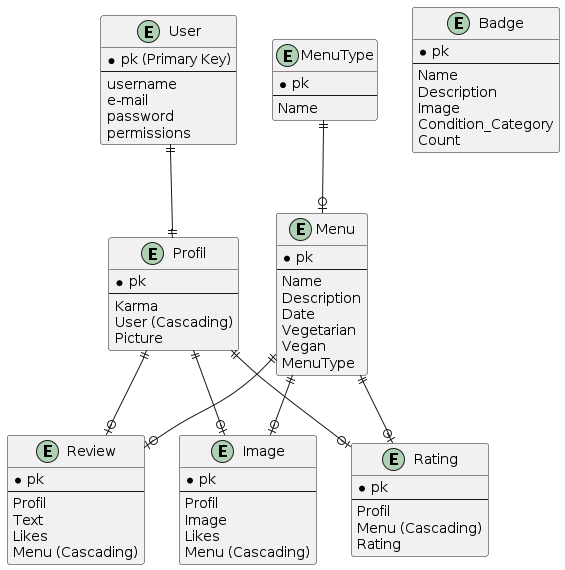
\includegraphics[width=0.8\textwidth]{images/Database.png}
    \caption{Architektur der Datenbank siehe auch \ref{code:models.py}}
    \label{fig:DB}
\end{figure}

\subsection{Architektur der Webseite}
\begin{figure}[ht]
    \centering
    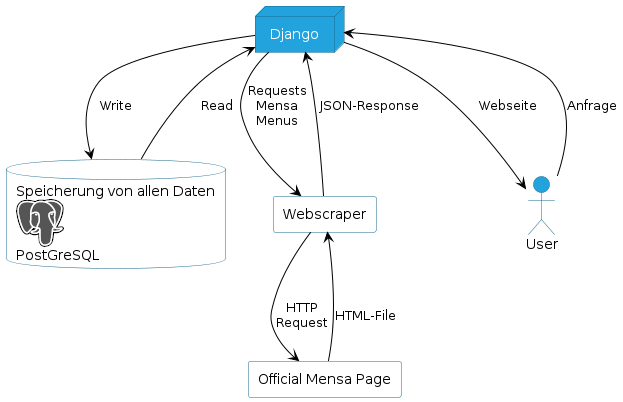
\includegraphics[width=0.8\textwidth]{images/Webseite.png}
    \caption{Architektur der Webseite}
    \label{fig:Website}
\end{figure}

\section{Problemdefinition}\label{sec:problemdefinition}

Die Grundanforderung für das Projekt sind:
\begin{itemize}
    \item Menus von der Mensa müssen geladen werden und angezeigt werden
    \item Bilder Gallerie, wo man die Bilder der Gerichte sehen, posten und liken kann
    \item Reviews vom Essen müssen gepostet, geliked und gesehen werden
    \item Das Essen muss mit einem Rating bewertet werden können
    \item Die Menus müssen nach verschiedene Kriterien sortiert/gefiltert werden können.
    \item Die Webseite braucht ein ansprechendes und einfaches Design
\end{itemize}

Damit das Projekt noch erfolgreicher wird, braucht es:
\begin{itemize}
    \item Account System
    \item Mobile Responsiveness für eine gute Nutzung auf Smartphones
    \item Subkommentare für Reviews
    \item Ein Punktesystem (Karma) für qualitative Bewertungen
    \item Eine Veröffentlichung auf eine richtige Serverinfrastruktur
\end{itemize}

\chapter{Spezifikationen}

\section{Use Cases} \label{sec:UseCases}
\begin{figure}[ht!]
    \centering
    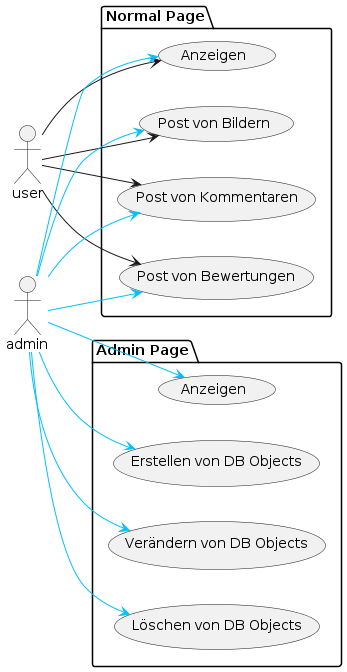
\includegraphics[width=0.45\textwidth]{images/Use Case.png}
    \caption{Use Cases}
    \label{fig:UseCases}
\end{figure}

\newpage

\section{Anforderungen} \label{sec:Anforderungen}
\subsection{Menus} \label{spez:Menus}

Menus sind Objekte, welche in der Datenbank als \code{Menu}-Objekt gespeichert
werden (siehe \ref{fig:DB}, \ref{code:core.models.py}). Jedes \code{Menu} ist
ein Vorkommen eines Gerichts. Um die verschiedenen Vorkommen der
\code{Menu}-Objekte zu gruppieren existiert das \code{MenuType}-Objekt.
Menus mit dem selben Namen wird der gleiche \code{MenuType} zugeordnet.

Die Menus werden von der Mensa-Website gescraped. Die Synchronization (siehe
\ref{spez:Webscraper}) findet bei jedem Aufruf einer der Seiten statt.

Nur wenn das heutige Datum mit dem Datum des Menus übereinstimmt, ist es
möglich, Bilder zu posten (siehe \ref{spez:Images}), das Menu zu bewerten (siehe
\ref{spez:Rating}) und die Posts zu liken (siehe \ref{spez:Liking}).

\subsection{Webscraper} \label{spez:Webscraper}

Der Webscraper ist ein standalone Python Script (siehe
\ref{code:core.webscraper.py}). Der Webscraper stellt mit der Library
\code{requests} Anfragen an die Webseite
\url{https://neuekanti.sv-restaurant.ch/de/menuplan/}. Zuerst werden die Tages-
und Datumsdaten von der Seite geladen. Danach werden die Gerichte (Name,
Beschreibung, Vegan/Vegetarisch) gescraped.

% TODO: Dringens mit den neuen Änderungen umschreiben

Das Script wird bei jedem Aufruf der Webseite ausgeführt. Nach dem Scraping
der Daten werden diese mit der Datenbank (siehe \ref{fig:DB}) verglichen.
Ist das \code{Menu}-Objekt (siehe \ref{spez:Menus}) noch nicht in der Datenbank,
so wird nach einem zugehörigen \code{MenuType} (siehe \ref{spez:Menus})
gesucht. Wenn dieses nicht existiert, dann werden beide Objekte einfach mit den
Daten erstellt. Sonst wird nur das \code{Menu}-Objekt erstellt.

\newpage

\begin{lstlisting}
    data = scrape_data()
    for menu, date in data:
        menus = get_menus_from_db(date=date)
        if menu not in menus:
            menu_type = get_menu_type(menu=menu)
            if menu_type == null:
                menu_type = create_menu_type(menu, data)
            create_menu(data, menu_type)
\end{lstlisting}

(Code in \code{core/webscraper.py})

\subsection{Bilder Gallerie} \label{spez:Gallerie}

Die Bildergallerie ist ein Frontend Feature. Die Bildergallerie wurde von dem
Tutorial auf dieser Seite nachgemacht:
\url{https://www.w3schools.com/howto/howto_js_slideshow.asp}. Die Bildergallerie
wird gebraucht, damit die Images (siehe \ref{spez:Images}) der Menus (siehe
\ref{spez:Menus}) angezeigt werden können.

Im Javascript werden die verschiedenen Bilder in einem Array gespeichert. Nur
das aktive Bild bekommt den style \code{display: block}. Die anderen Bilder
haben \code{display: none}.

Wenn es noch keine Bilder von einem Menu gibt, dann wird ein default Bild
angezeigt.

Da Bilder Hoch- oder Querformat sein können, werden sie auf ihre Orientierung
überprüft. Wenn das Bild Hochformat ist, dann wird es im css anders
behandelt.

\subsection{Posts} \label{spez:Posts}

Der Begriff "Posts" beschreibt zwei verschiedene Objekte in der Datenbank (siehe
\ref{fig:DB}). Es gibt kein übergeordnetes Objekt Posts. Als Posts werden Images
(siehe \ref{spez:Images}) und Reviews (siehe \ref{spez:Reviews}) bezeichnet.

Ein Post, sowie eine Bewertung (siehe \ref{spez:Rating}), kann nur gemacht
werden, wenn das zugehörige \code{Menu} von heute ist. Man kann auch nur die
Posts von dem heutigen Tag liken (siehe \ref{spez:Liking}).

Um einen Post zu schicken, schickt man ein \code{POST-HTML-Form} an das Backend.
Auch im \code{Menu}-View (siehe menu bei {\ref{code:core.views.py}}) wird die
Anfrage verarbeitet. Es wird ausgewertet, was für eine Art Post es ist und es
wird sich dann spezifisch in den \code{post\_function.py} dann um das Speichern
und genauere Auswerten des Formulars gekümmert. Danach wird noch eine
Rückmeldung (\code{message}) an den User gesendet.

\subsubsection{Images} \label{spez:Images}

Es gibt ein \code{Image}-Objekt in der Datenbank (siehe \ref{fig:DB} und in
\ref{code:core.models.py}). Die Image Datei wird nicht in der Datenbank
gespeichert, lediglich eine Referenz, welche auf das Bild verweist.

Wenn das Image auf der öffentlichen Webseite (siehe \ref{spez:Deployment}) angezeigt wird, dann
wird das Image nicht auf dem eigentlichen Server gespeichert, sondern auf einem
Google Drive. Das wird gemacht, da der Server Container keinen persistant
Storage hat.

\subsubsection{Reviews} \label{spez:Reviews}

Es gibt ein \code{Review}-Objekt in der Datenbank (siehe \ref{fig:DB} und in
\ref{code:core.models.py}). Ein Review ist ein Kommentar zu einem Menu
(\ref{spez:Menus}), welcher auf der Webseite angezeigt werden kann.

\subsubsection{Liking} \label{spez:Liking}

Man kann die Posts liken. Dabei wird der Like Counter in der Datenbank (siehe
\ref{fig:DB} und in \ref{code:core.models.py}) erhöht. Ob der User bereits
geliked hat, wird im Javascript Localstorage gespeichert. Die Likes werden nicht
in seperaten Objekten gespeichert, damit die Datenbank nicht zu viele Einträge
bekommt.

Das Liking wird im Javascript gemacht. Die Information wird von dort ins Backend
(siehe like bei \ref{code:core.views.py}) geschickt und dort in der Datenbank
gespeichert. Währenddessen wird der Like Status im Localstorage gespeichert.
Sobald die Anfrage zurückkommt, wird der Like Counter aktualisiert.

\subsection{Rating} \label{spez:Rating}

Ein Rating ist ein Objekt in der Datenbank (siehe \ref{fig:DB} und in
\ref{code:core.models.py}). Ein Rating ist eine Bewertung für ein Menu-Objekt
(siehe \ref{spez:Menus}). Ein Rating hat einen Wert zwischen 1 und 5.

Diese werden auf der Webseite zusammengezählt und der Durchschnitt berechnet,
damit sie auf der Webseite angezeigt werden können.


\subsection{Statistik: Filter und Sortierung} \label{spez:Statistik}

Auflistungen von Menus können gefiltert und sortiert werden. Folgende Filter
können durch einen Button ausgewählt werden: nur vegan, nur vegetarisch und kein
Filter. Folgende Sortierungen können durch einen Button ausgewählt werden:
Rating-Durchschnitt (absteigend), Alphabetisch, Anzahl Ratings und Anzahl
Vorkommen (letzteres nur unter der Seite `alle Menus', weil nur \code{MenuType}
Objekte dieses die Möglichkeit so etwas zu besitzen haben).

Beim Neuladen der Seite werden die Daten aller Menus in der Auflistung aus der
Datenbank gesammelt (bei der Seite `alle Menus' (siehe \ref{code:core.views.py})
werden alle \code{MenuType}-Objekte anstelle der Menus angezeigt) und
standardmässig nach dem Rating-Durchschnitt sortiert. 

Das Filtern und Sortieren auf Knopfdruck erfolgt in Javascript. Die einzelnen
\code{<div>} Elemente im HTML Code, die ein Element der Auflistung beschreiben,
sind standardmässig leer und werden durch die Javascript Funktion
\code{updateListboxs()} mit den Daten der Menus oder MenuTypes gefüllt. Diese Daten sind pro
Menu in einem Javascript Object gespeichert:

\begin{lstlisting}
    menuType = {
        url: data.url,
        name: data.name,
        index: data.index,
        rating: data.rating,
        occurrences: data.occ,
        numrates: data.numrates,
        vegan: data.vegan,
        vegetarian: data.vegetarian,
        visible: true
    }
\end{lstlisting}

(Code in \code{core/templates/allMenu.html})

Je nach Filter wird das visible Attribut auf \code{false} gesetzt, wodurch die
Daten des zugehörigen Menus oder MenuTypes in der Auflistung nicht mehr
angezeigt werden. Das passiert ebenfalls durch die \code{updateListboxs()} Funktion

\newpage

\subsection{Account System} \label{spez:Account}

Die Entwicklung des Accountsystems ist stark von der diesem Django inspiriert
(\url{https://www.youtube.com/playlist?list=PL-osiE80TeTtoQCKZ03TU5fNfx2UY6U4p}).
Allerdings wurde der Code in verschiedenen Projekten bereits verwendet und
dadurch immer weiter entwickelt und vom Tutorial unabhängig gemacht.

Django hat ein eingebautes Accountsystem. Dieses Accountsystem wird in die
Webseite integriert (siehe \ref{code:users.views.py}). Es bietet folgende
Funktionen:
\begin{itemize}
    \item register
    \item login
    \item logout
    \item password-reset
    \item password-reset-done
    \item password-reset-confirm
    \item password-reset-complete
\end{itemize}

Beim Registrieren wird ein \code{User}-Objekt in der Datenbank (noch nicht in der
models.py Datei) erstellt. Danach auch ein \code{Profil}-Objekt (siehe
\ref{code:core.models.py} und \ref{fig:DB}). Beim Registrieren gibt es auch noch
eine ReCaptcha-Überprüfung, damit die Datenbank nicht zugespammt werden kann. Eine Email-Verifikation gibt es nicht

Login und Logout verwalten die Session mit den von Django implementierten
Funktionen.

Die Funktion des Passwordresets funktioniert über die angegebene Email Adresse.
Es wird ein sicherer Token für den Passwordreset an die Email Adresse gesendet.
Die Email wird über einen Gmail Account versendet.

\subsection{Mobile Responsiveness} \label{spez:Mobile}

In Milestone 1 noch nicht implementiert.

\subsection{Punktesystem (Karma)} \label{spez:Karma}

Die Erfahrungspunkte, auch Karma genannt, werden in \code{Profil}-Objekt (siehe
\ref{fig:DB} und \ref{code:core.models.py}) gespeichert.

Man kann Punkte für das Veröffentlichen von Posts (siehe \ref{spez:Posts}) und für
Likes auf den eigenen Posts bekommen. (Funktion \code{add\_karma\_for\_posting})

Mit den Punkten kann man Achievements erreichen (siehe \ref{spez:Badges}).

\subsection{Achievements (Badges)} \label{spez:Badges}

Die Achievements werden als \code{Badge}-Objekt in der Datenbank (siehe \ref{fig:DB} und in
\ref{code:core.models.py}) gespeichert. Die Objekte werden keinem User
zugeordnet gespeichert, sondern dynamisch berechnet, wer welche Achievements
hat.

\begin{lstlisting}
    def get_badges_of_profil(profil):
        badges = Badge.objects.all()

        img_counter = count_best_image_of_profil(profil=profil)
        review_counter = count_best_review_of_profil(profil=profil)
        karma = profil.karma

        categories = [karma, img_counter, review_counter]

        highest_badge = [null, null, null]
        for i in badges:
            if i.count <= categories[i.condition_category]:  # Does the profil own the badge?
                if highest_badge[i.condition_category] is null:
                    highest_badge[i.condition_category] = i
                else:
                    if highest_badge[i.condition_category].count < i.count:
                        highest_badge[i.condition_category] = i
        
        highest_badges = [i for i in highest_badges if i is not None]  # Remove null badges
\end{lstlisting}

(Code in \code{core/statisticFunctions.py})



Es gibt 3 verschiedene Kategorien von Achievements.
\begin{itemize}
    \item Karma-basiert (siehe \ref{spez:Karma})
    \item Images-basiert (siehe \ref{spez:Images})
    \item Review-basiert (siehe \ref{spez:Reviews})
\end{itemize}

Wenn man ein besseres Achievements in einer Kategorie erreicht, dann wird das
alte durch das neue ersetzt. Man kann Achievements auch wieder verlieren, wenn
man die Kriterien nicht mehr erfüllt.

Karma-basiert heisst, man bekommt ein Achievment in dieser Kategorie, wenn man
eine bestimmte Menge an Karma überschritten hat.

Image- und Review-basiert heisst, dass man eine bestimmte Anzahl an `most liked
Images/Reviews' in einem MenuType (siehe \ref{spez:Menus}) hat.

Alle erreichten Achievements sind im Profil ersichtlich (siehe \ref{code:core.views.py})

\subsection{Deployment} \label{spez:Deployment}

Die Webseite wird auf einem Heroku Eco Dyno gehostet. Die Datenbank wird ebenfalls
von Heroku auf einem Postgres Server gehostet. Die Bilder werden auf einem
Google Drive gespeichert (siehe \ref{spez:Images}).

Heroku wurde für dieses Projekt gewählt, weil es eine sehr einfache
\code{Django} Deployment Plattform ist und es sehr viele Anleitung im Internet
gibt. Heroku beitet weiter auch noch viele Addons, welche für
Weiterentwicklungen und Veröffentlichungen nützlich sein könnten. Ausserdem
wurden in vergangenen Projekten gute Erfahrungen mit Heroku gemacht, weswegen
die Wahl auf diesen Anbieter fiel.

\chapter{Entwurf} \label{chap:entwurf}

\section{Architektur der Datenbank} \label{sec:DB}
\begin{figure}[ht]
    \centering
    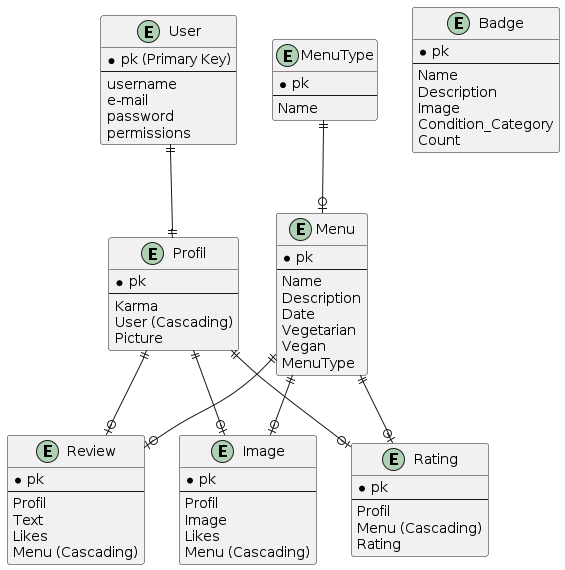
\includegraphics[width=0.8\textwidth]{images/Database.png}
    \caption{Architektur der Datenbank siehe auch \ref{code:core.models.py}}
    \label{fig:DB}
\end{figure}

Diese Skizze repräsentiert den Aufbau der Datenbank. Sie zeigt die verschiedenen
Entitiys und ihre Beziehungen. Die Datenbankstruktur ist in der Datei
\code{core/models.py} beschrieben (siehe \ref{code:core.models.py}).

\section{UML-Diagramm der WebApp} \label{sec:UMLS}
\begin{figure}[ht]
    \centering
    
\includegraphics[width=0.4\textwidth]{images/UML-Specific.png}
    \caption{UML Diagramm der WebApp}
    \label{fig:DB}
\end{figure}

Dieses UML-Diagramm zeigt die Zusammenhänge aller Komponenten (nicht Klassen,
häufig einfach Funktine) der WebApp. Dabei sind nur die Verbindungen der
\code{Index} Seite und der \code{Menu} Seite vorhanden, da es mit allen
Verbindungen zu unübersichtlich werden würde.

\newpage

\section{Vereinfachtes UML-Diagramm der WebApp} \label{sec:UMLG}
\begin{figure}[ht]
    \centering
    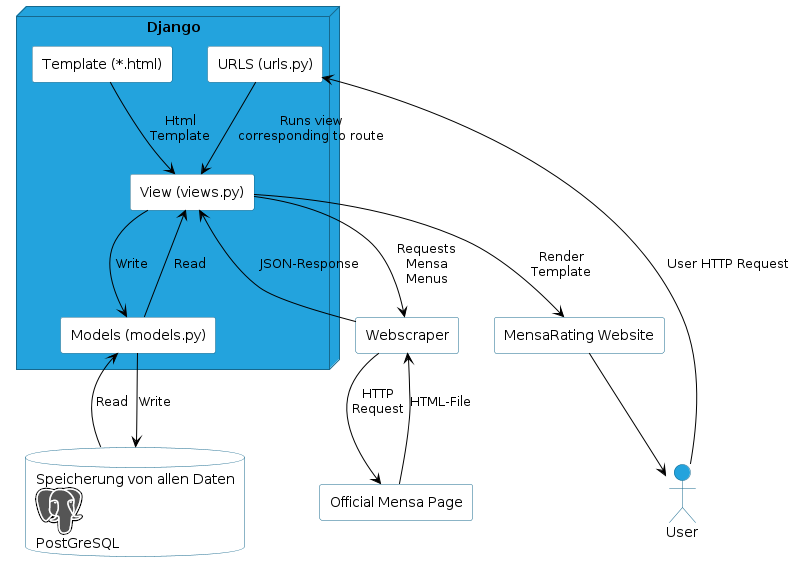
\includegraphics[width=0.8\textwidth]{images/UML-General.png}
    \caption{UML Diagramm (vereinfacht) der WebApp}
    \label{fig:DB}
\end{figure}

Dieses UML diagramm ist weniger spezifisch als das letzte (siehe
\ref{sec:UMLS}). Im Gegensatz zum letzten Diagramm zeigt dieses allerdings alle
wichtigen Verbindungen der einzelnen Komponenten der WebApp (Django, die
Datenbank, die Webseite, die offizielle Mensa Webseite und der User)



\chapter{Resultate und Testen} \label{chap:resultate}

\section{Testen} \label{sec:testen}

Die Webseite lässt in einer lokalen Entwicklungsumgebung oder auf der
öffentlichen Seite testen. Getestet wurden die Funktionen manuell von Hand oder
auch teilweise durch automatisierte Tests.

Grundsätzlich funktionieren alle Funktionen. Schlussendlich gibt es nur ein
Problem: Es kommt vor, dass der Webscraper Edge-Cases antrifft. Das kann
passieren, wenn die offizielle Mensa Webseite die Informationen auf ihrer
Webseite kurzfristig ändern. Es wurde versucht diese Edge-Cases möglichst alle
abzufangen, allerdings kann es immer noch sein, dass es manchmal zu Fehlern
kommt und die Daten der Webseite sich von der offiziellen Webseite
unterscheiden. Diese Fehler müssen jeweils von einem Admin auf der Admin-Seite
behoben werden.

\section{Resultate} \label{sec:resultate}

Das Resultat dieser Webseite ist eine voll Funktionstüchtige Webseite
Die Webseite erfüllt alle nötigen Anforderungen (siehe
\ref{sec:problemdefinition}). Die Webseite ist auch öffentlich zugänglich
(siehe \ref{spez:Deployment}) und kann unter
\url{http://mensarating.herokuapp.com/} aufgerufen werden. 
\subsection{Resultate der Grundanforderungen}
 
\newpage

\subsubsection*{Anzeige der Menus}

\begin{figure}[ht]
    \centering
    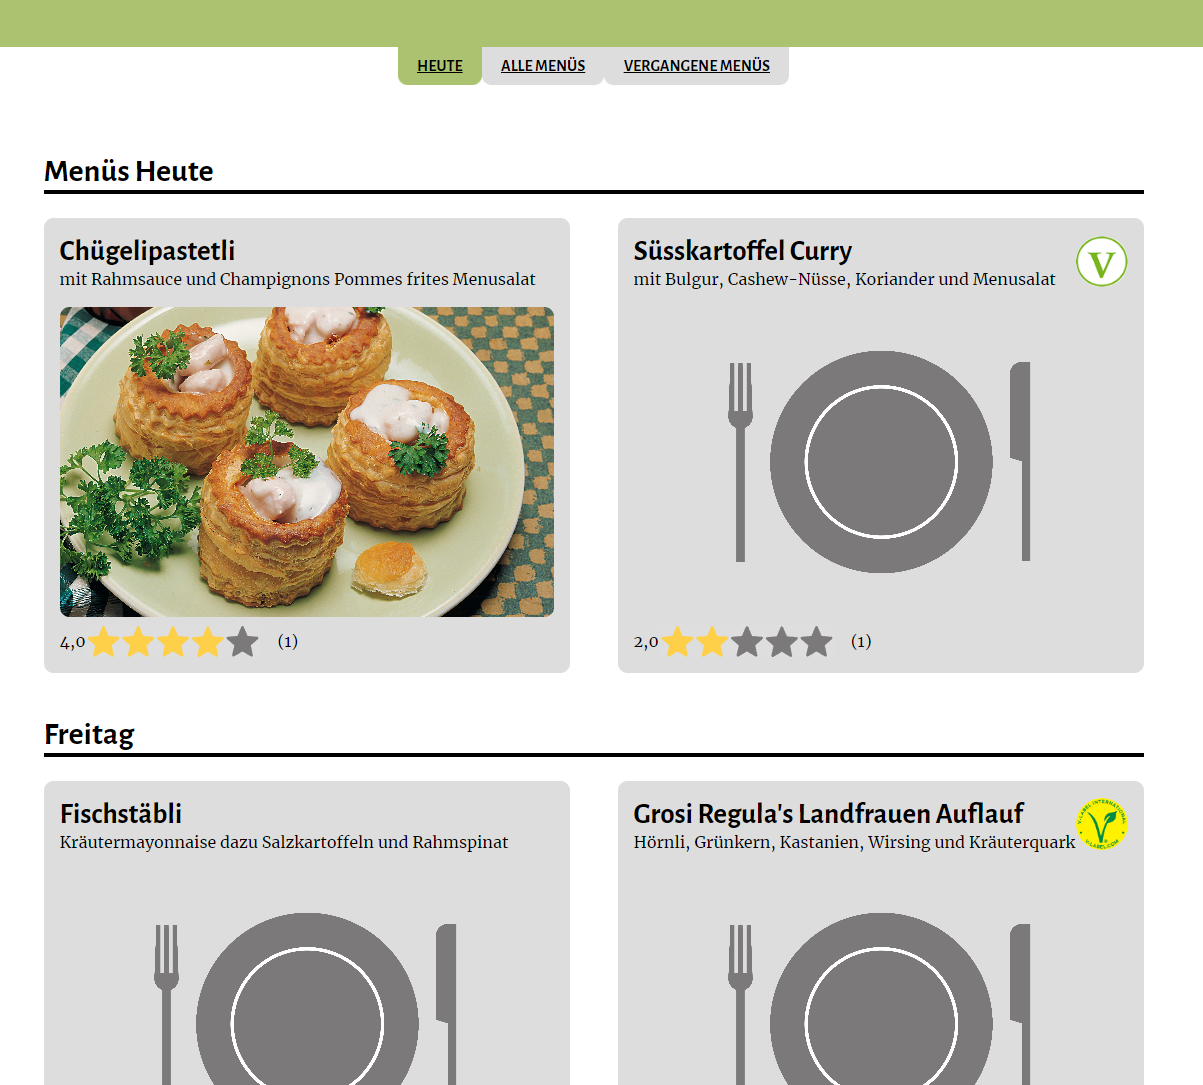
\includegraphics[width=0.8\textwidth]{images/Resultate_Menu.png}
    \caption{Screenshot: Anzeige Menus auf Startseite}
    \label{fig:r-menuindex}
\end{figure}

Auf der Startseite der Webseite (siehe \ref{fig:r-menuindex}) werden die beiden Menus des Tages, die von der
offiziellen Mensa Webseite gescraped wurden, angezeigt. Es wird die
Beschreibung, ein Label (Vegan/Vegetarisch), das durchschnittliche Rating und
das Bild mit den meisten Likes angezeigt. Als Zusatz sind die zukünftigen Menus
ebenfalls angezeigt.

\begin{figure}[htp]
    \begin{subfigure}[b]{0.5\textwidth}
        \centering
        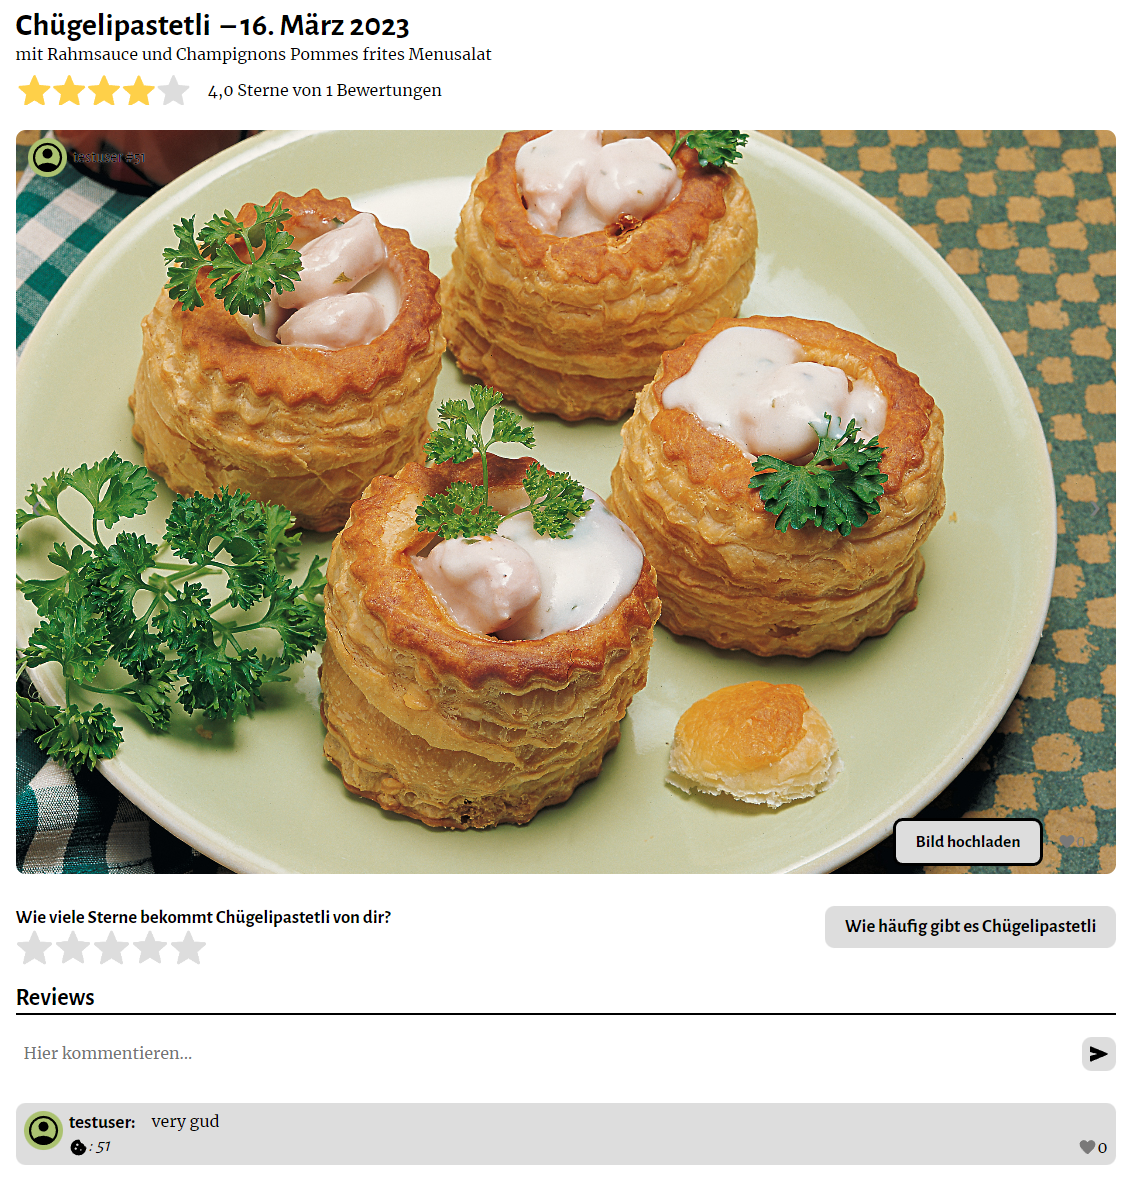
\includegraphics[width=0.7\textwidth]{images/Res_Menu.png}
        \caption{Screenshot: Menu Web Page}
        \label{fig:r-menu}
    \end{subfigure}
    \begin{subfigure}[b]{0.5\textwidth}
        \centering
        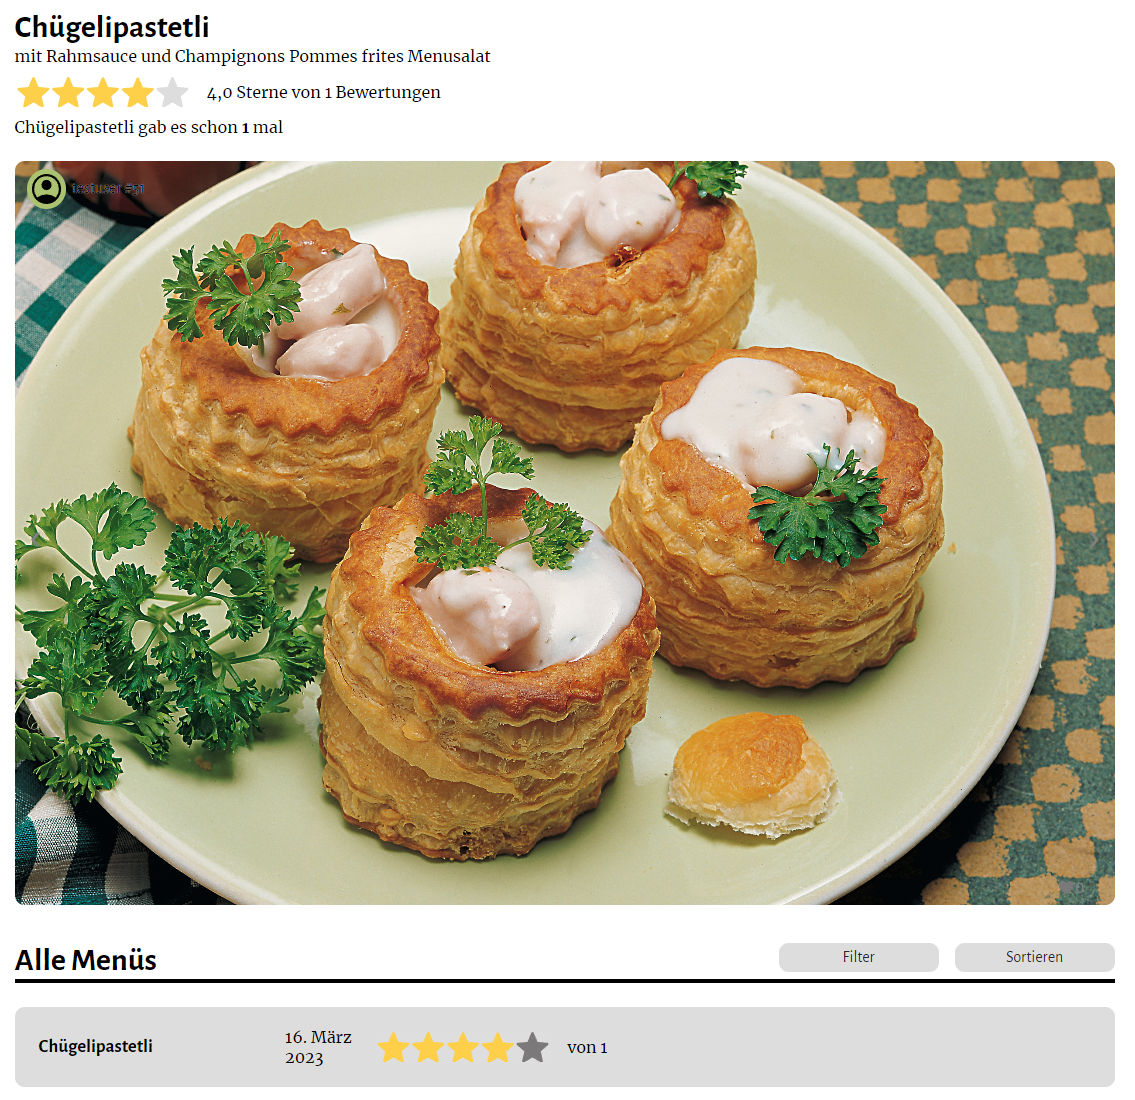
\includegraphics[width=0.7\textwidth]{images/Res_Menutype.png}
        \caption{Screenshot: Menutype Web Page}
        \label{fig:r-menutype}
    \end{subfigure}
    \hfill
\end{figure}

Zusätzlich gibt es eine Menu Page (siehe \ref{fig:r-menu}) und eine MenuType
Page (siehe \ref{fig:r-menutype}), wo die Menus genauer angezeigt werden  


\subsubsection*{Bilder Gallerie}

\begin{figure}[htp]
    \begin{subfigure}[b]{0.5\textwidth}
        \centering
        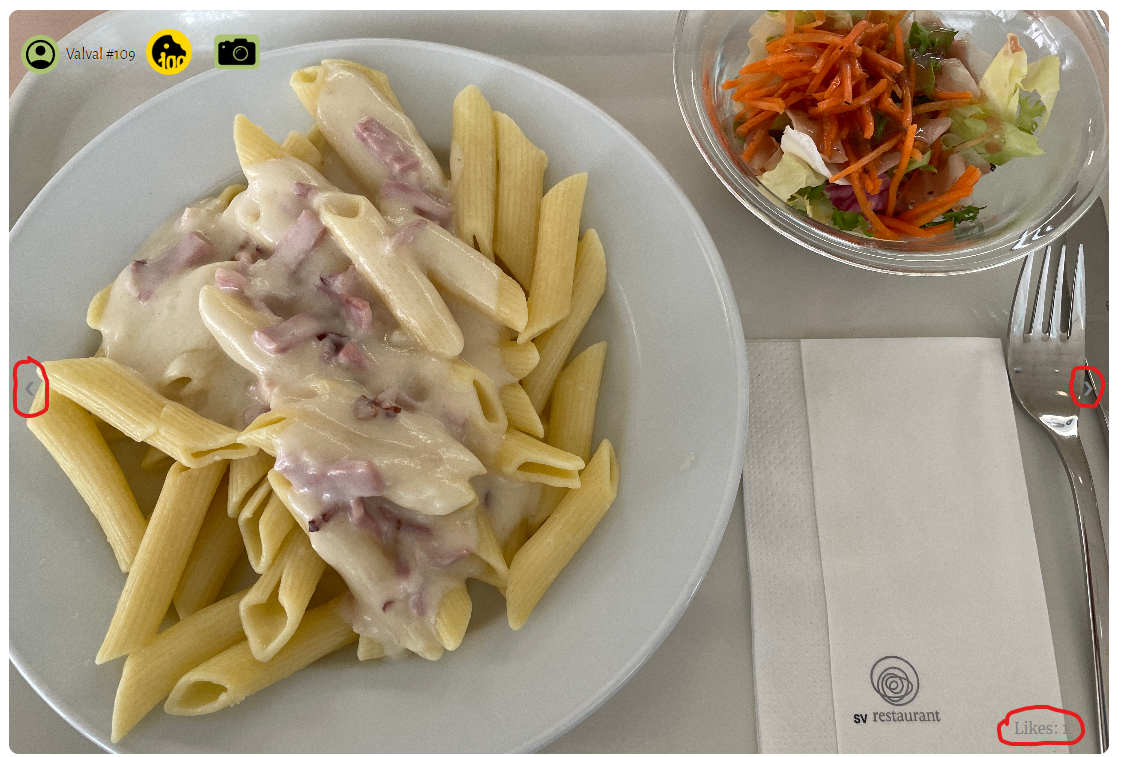
\includegraphics[width=0.7\textwidth]{images/Resultate_Bildergallerie.png}
        \caption{Screenshot: Bildergallerie}
        \label{fig:r-bildergallerie}
    \end{subfigure}
    \begin{subfigure}[b]{0.5\textwidth}
        \centering
        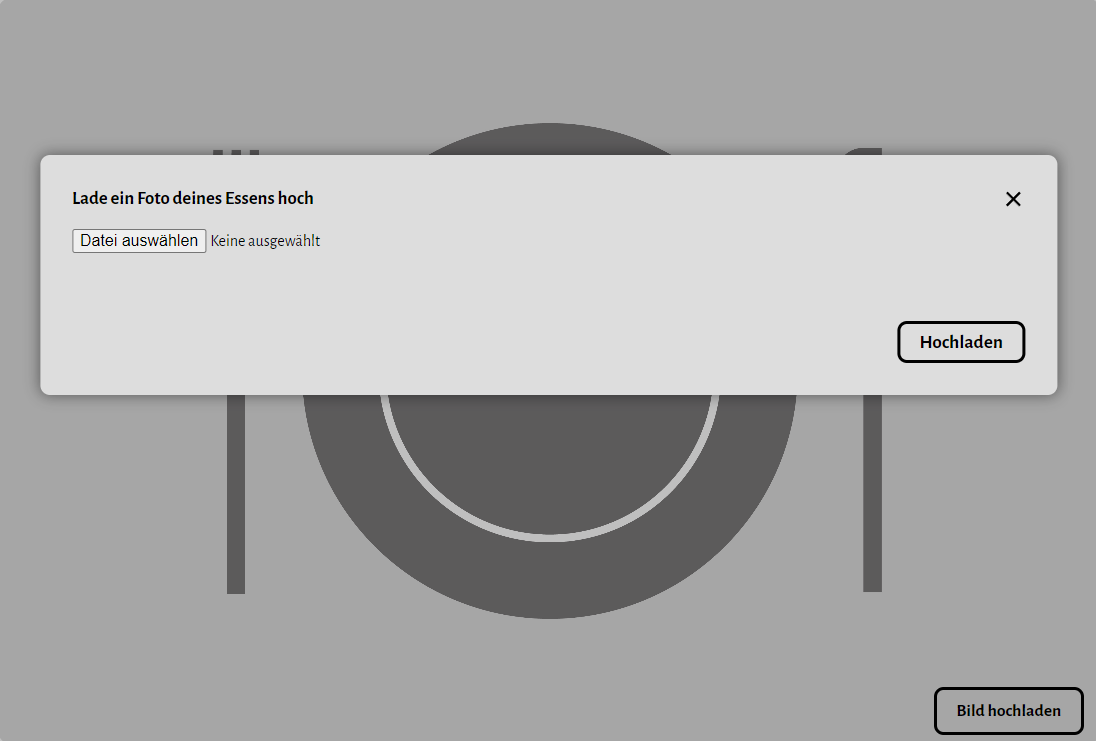
\includegraphics[width=0.7\textwidth]{images/Resultat_Bildergallerie_upload.png}
        \caption{Screenshot: Bilder Upload}
        \label{fig:r-bildpopup}
    \end{subfigure}
    \hfill
\end{figure}

Bei der Bildergallerie (siehe \ref{fig:r-bildergallerie}) können User Bilder
hochladen. Man kann durch Pfeil-Buttons die verschiedenen hochgeladenen Bilder
ansehen. Für jedes Bild ist erstens der User angezeigt, der es hochgeladen hat, und zweitens die
Anzahl Likes. Der Upload findet über einen Upload Button statt, der ein Pop-Up
öffnet (siehe \ref{fig:r-bildpopup})


\subsubsection*{Reviews}

\begin{figure}[ht]
    \centering
    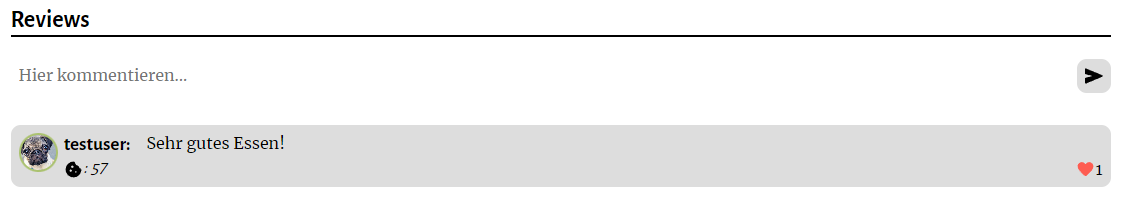
\includegraphics[width=0.8\textwidth]{images/Resultat_Review.png}
    \caption{Screenshot: Veröffentlichung und Anzeige von Reviews}
    \label{fig:r-review}
\end{figure}

Am Tag, an dem es ein bestimmtes Menu gibt, kann diesem Menu ein Review (siehe
\ref{fig:r-review}) gegeben werden. Die Reviews sind in einer Liste angeordet
und bei jedem Review ist der User angegeben, zusammen mit seinen Achievements
und Karma Punkten. Reviews können geliked werden (beachte das Herz).

\subsubsection*{Rating}

\begin{figure}[ht]
    \centering
    
\includegraphics[width=0.8\textwidth]{images/Resultat_Rating.png}
    \caption{Screenshot: Anzeige vom Rating eines Menus}
    \label{fig:r-rating}
\end{figure}

Ein User kann einem Menu als Rating einen bis fünf Sterne gebe. Der User drückt
dabei auf die Anzahl Sterne, die er geben will. Der Durchschnitt des Ratings
wird ebenfalls in der Form von Sternen angezeigt. Dabei kann es auch nicht volle
Sterne geben (siehe \ref{fig:r-rating}) 

\subsubsection*{Filtern/Sortieren}

\begin{figure}[ht]
    \centering
    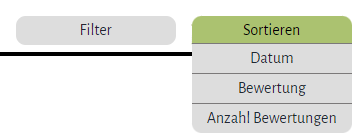
\includegraphics[width=0.8\textwidth]{images/Resultat_Filter.png}
    \caption{Screenshot: Buttons für Filter- und Sortier-Optionen}
    \label{fig:r-filtersort}
\end{figure}

auf der `Alle Menüs' Page und der `MenuType' Page können die Menüs/MenuTypes
nach verschiedenen Optionen in einem Dropdown-Menu (siehe
\ref{fig:r-filtersort}) gefiltert/sortiert werden. Nach der Auswahl wird die
Aktion ohne einen Reload der Seite ausgeführt.

\subsubsection*{Design}
Das Design ist an allen bisherigen Screenshots erkennbar. Als Akzentfarbe wurde
ein Grün gewählt, an vielen Formen sind die Ecken abgerundet und die
verschiedenen Aktionen auf der Webseite sollten für den User so einfach wie
möglich gestaltet sein.

\newpage

\subsection{Resultate der Erweiterungskriterien}

\subsubsection*{Account System}

\begin{figure}[htp]
    \begin{subfigure}[b]{0.32\textwidth}
        \centering
        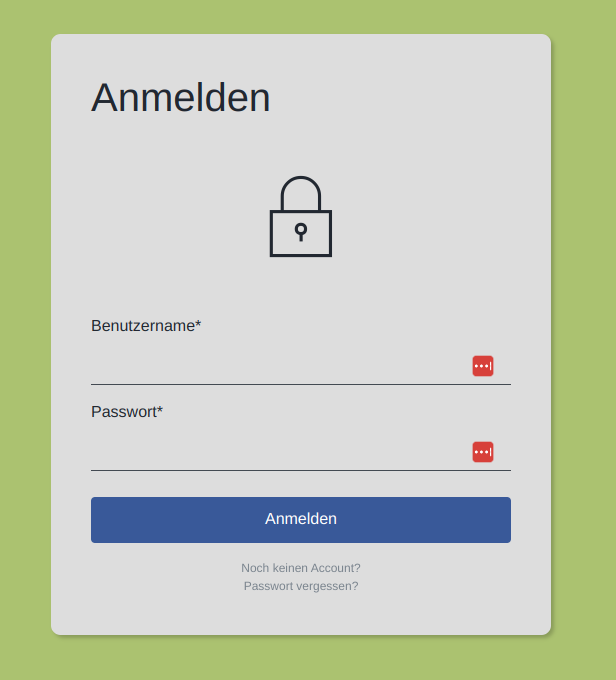
\includegraphics[width=0.7\textwidth]{images/Auth1.png}
        \caption{Screenshot: Login Form}
        \label{fig:r-login}
    \end{subfigure}
    \begin{subfigure}[b]{0.32\textwidth}
        \centering
        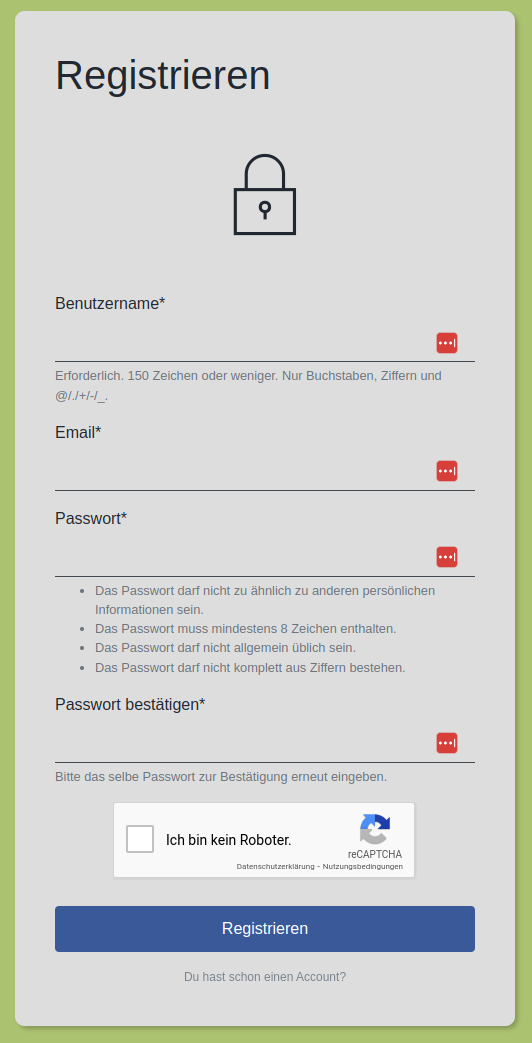
\includegraphics[width=0.5\textwidth]{images/Auth2.png}
        \caption{Screenshot: Registrieren Form}
        \label{fig:r-register}
    \end{subfigure}
    \begin{subfigure}[b]{0.32\textwidth}
        \centering
        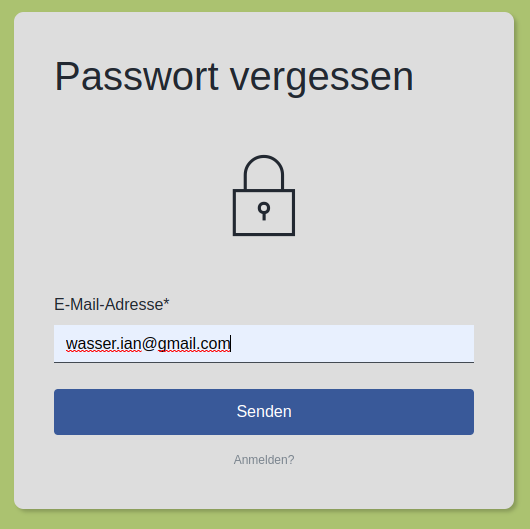
\includegraphics[width=0.7\textwidth]{images/Auth3.png}
        \caption{Screenshot: Passwort Reset Form}
        \label{fig:r-reset}
    \end{subfigure}
    \begin{subfigure}[b]{\textwidth}
        \centering
        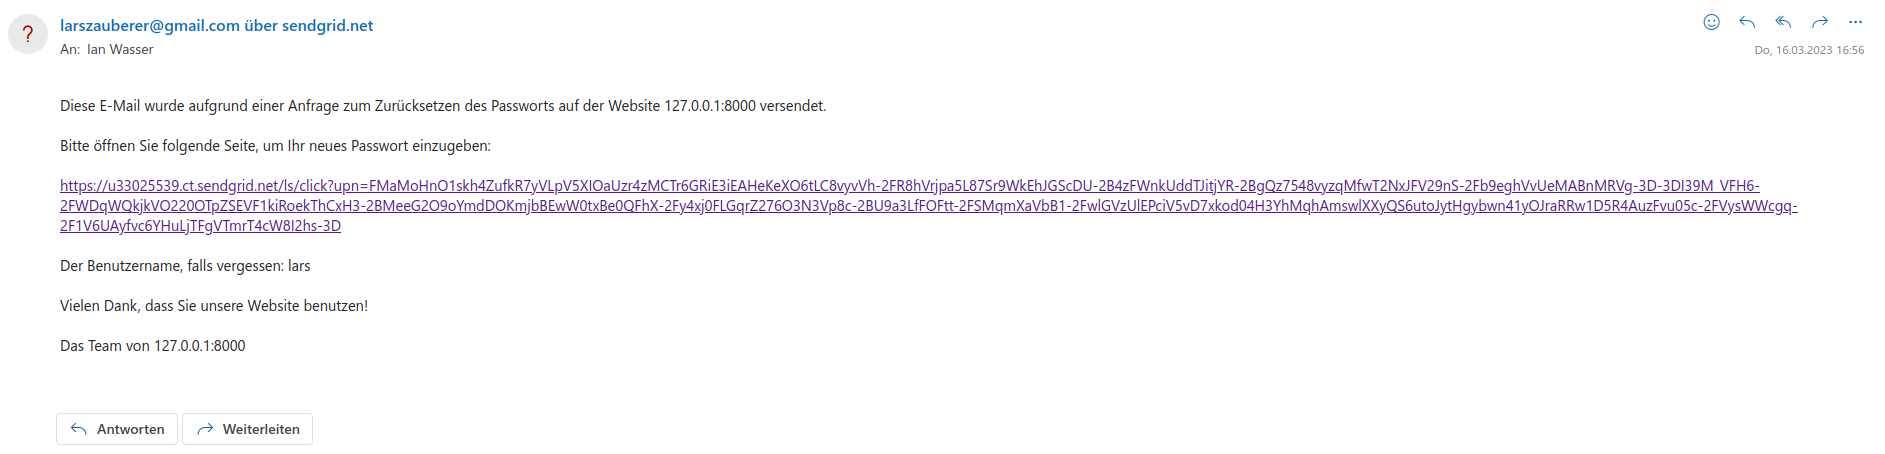
\includegraphics[width=\textwidth]{images/Auth4.png}
        \caption{Screenshot: Passwort Reset Mail}
        \label{fig:r-reset-mail}
    \end{subfigure}
    \begin{subfigure}[b]{\textwidth}
        \centering
        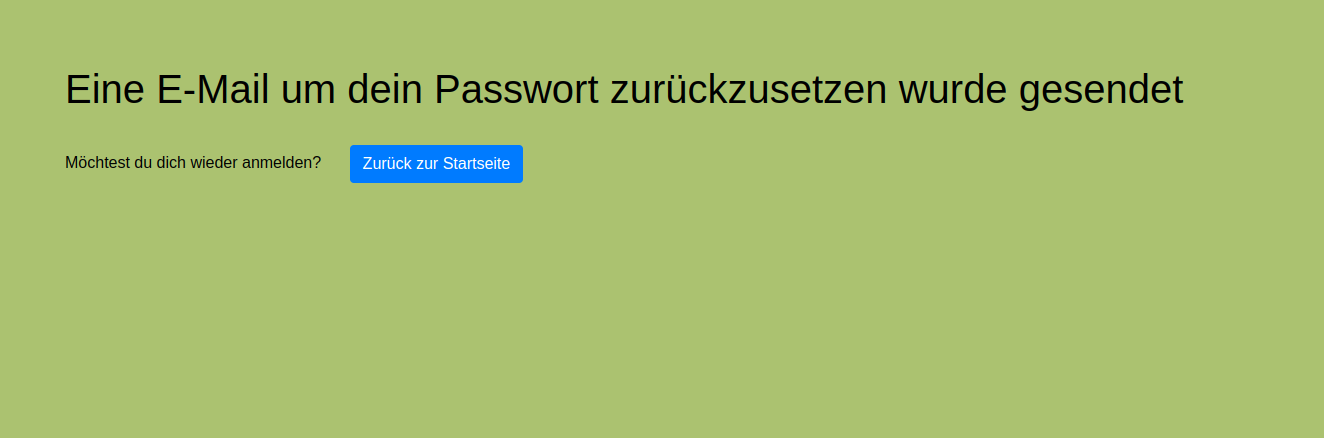
\includegraphics[width=\textwidth]{images/Auth5.png}
        \caption{Screenshot: Passwort Reset Complete}
        \label{fig:r-reset-complete}
    \end{subfigure}
    \caption{Screenshots: Account System}
    \label{fig:r-auth}
\end{figure} 

Die Webseite verfügt über ein komplett funktionierendes Account System. Wie den
einzelnen Screenshots zu entnehmen, kann der User sich registrieren, sich
einloggen, sich ausloggen und sein Passwort zurücksetzen.

\subsubsection*{Mobile Responsiveness}

\begin{figure}[ht]
    \centering
    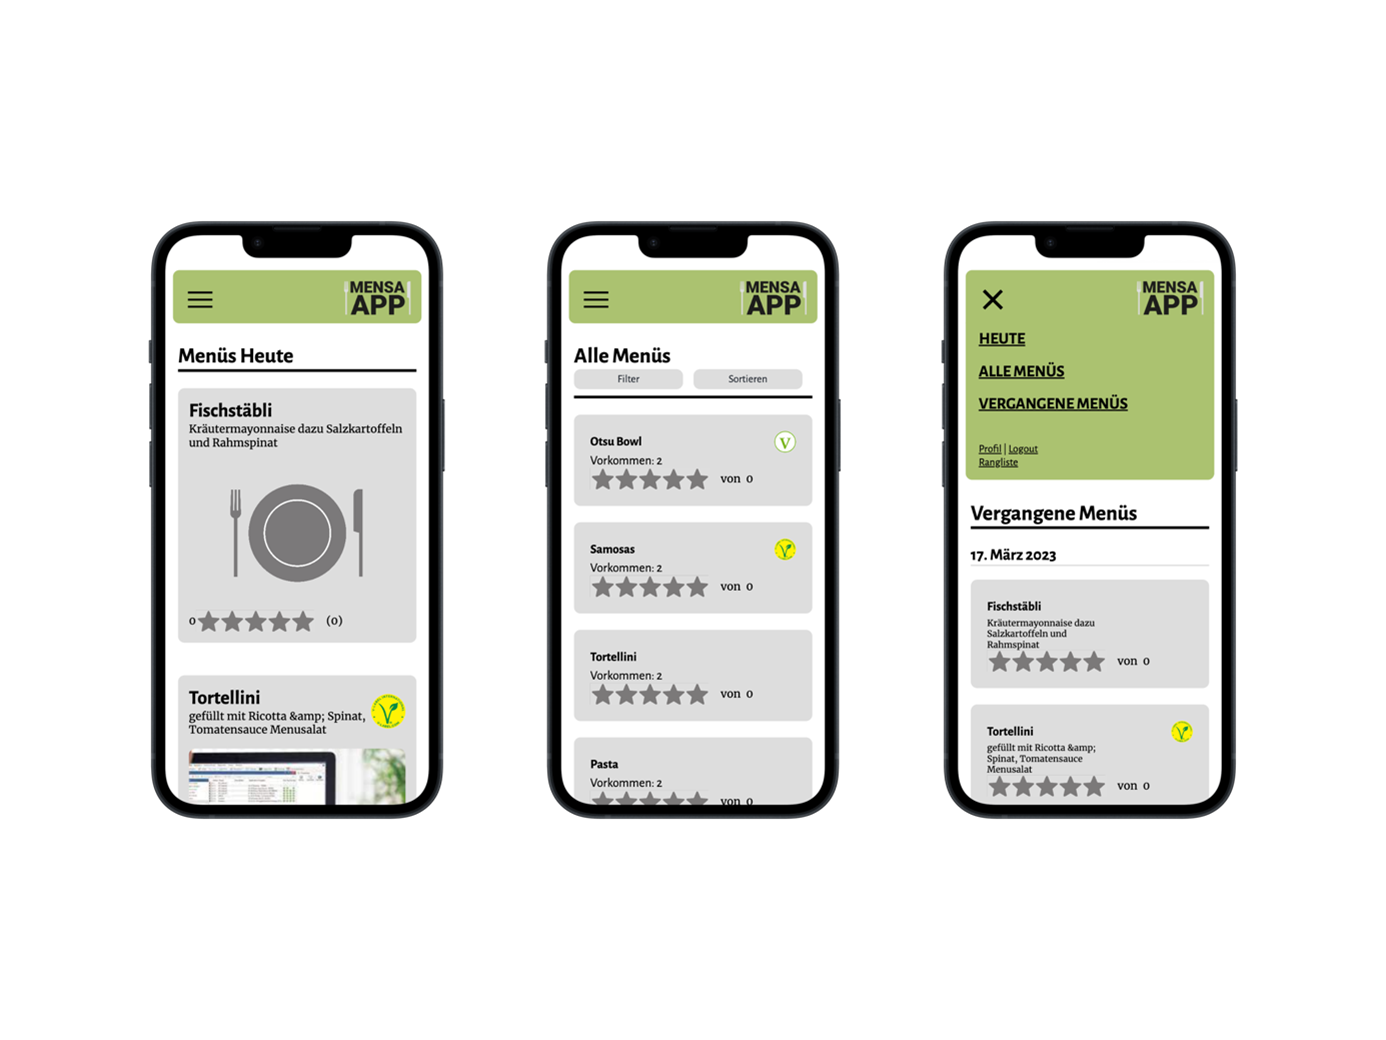
\includegraphics[width=0.8\textwidth]{images/Resultat_Responsive.png}
    \caption{Drei Beispiele der Mobile Responsiveness}
    \label{fig:r-karma}
\end{figure}

Beim Entwickeln der Website wurde davon ausgegangen, dass die meisten User mit
mobilen Endgeräten auf die Seite zugreifen. Daher ist es zentral, dass die
Website auf kleinen Bildschirmen einfach zu bedienen ist. Da ein Grossteil der
Seite mit Flexboxen designt wurde, war es meist einfach, den Inhalt für kleinere
Bildschirme anzupassen. Für andere Teile wurde ein komplett neues Design
erstellt, welches mithilfe von Media Queries nur auf kleinen Bildschirmen
dargestellt wird. Die Navigationselemente wurden komplett überarbeitet und
kleinere Seitenränder angewendet. Das Ziel, die Website Mobile Responsive zu
machen, wurde mit den oben erwähnten Schritten erreicht.


\subsubsection*{Punktesystem (Karma)}

\begin{figure}[ht]
    \centering
    
\includegraphics[width=0.5\textwidth]{images/Resultat_Karma.png}
    \caption{Screenshot: Karma eines Users (Auf Profilseite)}
    \label{fig:r-karma}
\end{figure}

User erhalten für Interaktionen auf der Webseite so genannte Cookiepoints (siehe
\ref{fig:r-karma}). Das Geben eines Ratings gibt einen Cookiepoint und das
Hochladen eines Bildes oder Reviews gibt 5 Cookiepoints. Wenn ein Post geliked
wird (siehe \ref{spez:Posts}), erhält der User, der geposted hat, einen
Cookiepoint. 

\begin{figure}[ht]
    \centering
    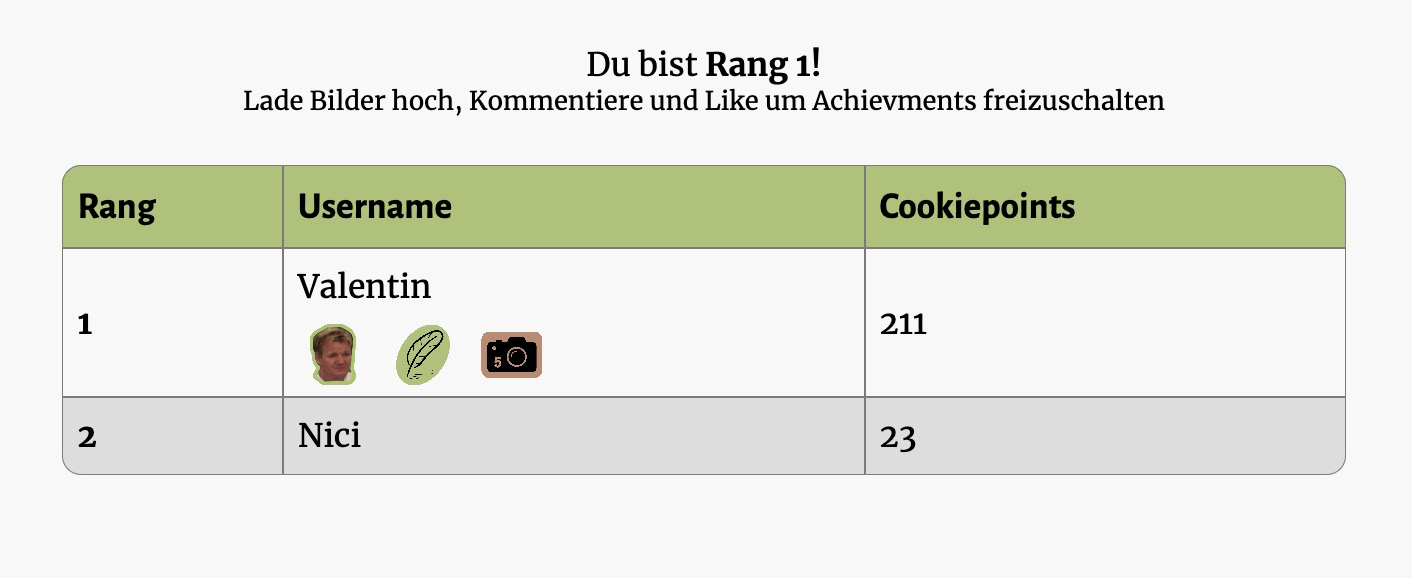
\includegraphics[width=0.8\textwidth]{images/Resultat_Rangliste.png}
    \caption{Screenshot: Karma Rangliste}
    \label{fig:r-rangliste}
\end{figure} 

Alle User mit Account sind in einer Rangliste aufgelistet. Die Rangliste bezieht
sich auf die Cookiepoints. Der User hat eine Angabe, wo er sich auf der
Rangliste befindet.

\subsubsection*{Achievement System}

\begin{figure}[ht]
    \centering
    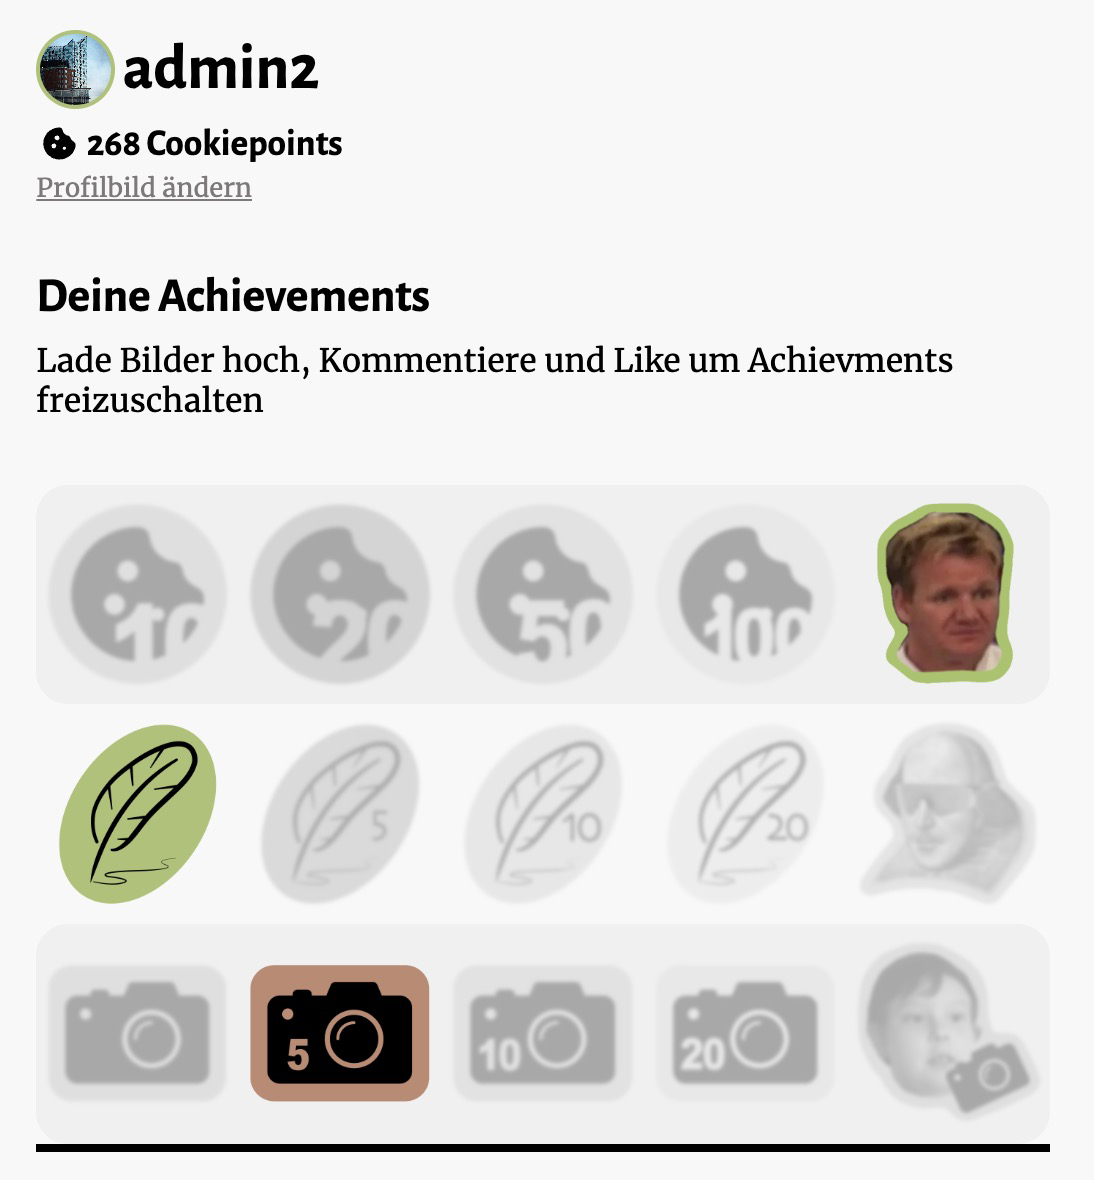
\includegraphics[width=0.8\textwidth]{images/Resultate_Achievements.png}
    \caption{Screenshot: Achievements Liste (Profil Page)}
    \label{fig:r-Achievement}
\end{figure} 

User können Achievements (siehe \ref{fig:r-Achievement}) erhalten. Die Bedinungen, um die Achievements zu
erhalten, sind in den Spezifikationen definiert (siehe \ref{spez:Badges}). Es
gibt fünf Achievements pro Kategorie. Wenn von einer Kategorie ein besseres
Achievement freigeschalten wird, wird dem User das Alte Achievement wieder
entzogen.

\begin{figure}[htp]
    \begin{subfigure}[b]{0.5\textwidth}
        \centering
        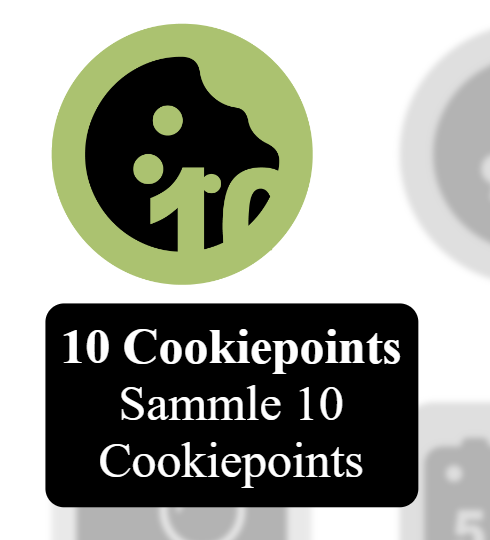
\includegraphics[width=0.7\textwidth]{images/Resultat-Beschreibung.png}
        \caption{Screenshot: Bildergallerie}
        \label{fig:r-Achievement-beschreibung}
    \end{subfigure}
    \begin{subfigure}[b]{0.5\textwidth}
        \centering
        
\includegraphics[width=0.7\textwidth]{images/Resultat-Username.png}
        \caption{Screenshot: Bilder Upload}
        \label{fig:r-username-display}
    \end{subfigure}
    \hfill
\end{figure}

Zu jedem Achievement gibt es eine kurze Beschreibung (siehe
\ref{fig:r-Achievement-beschreibung}), die angezeigt wird, wenn der User mit dem
Mauszeiger über dem Achievement hovered. Ausserdem werden die Achievements neben
dem User bei seinen Posts angezeigt (siehe \ref{fig:r-username-display}).

\newpage

\subsubsection*{Deployment}

\begin{figure}[ht]
    \centering
    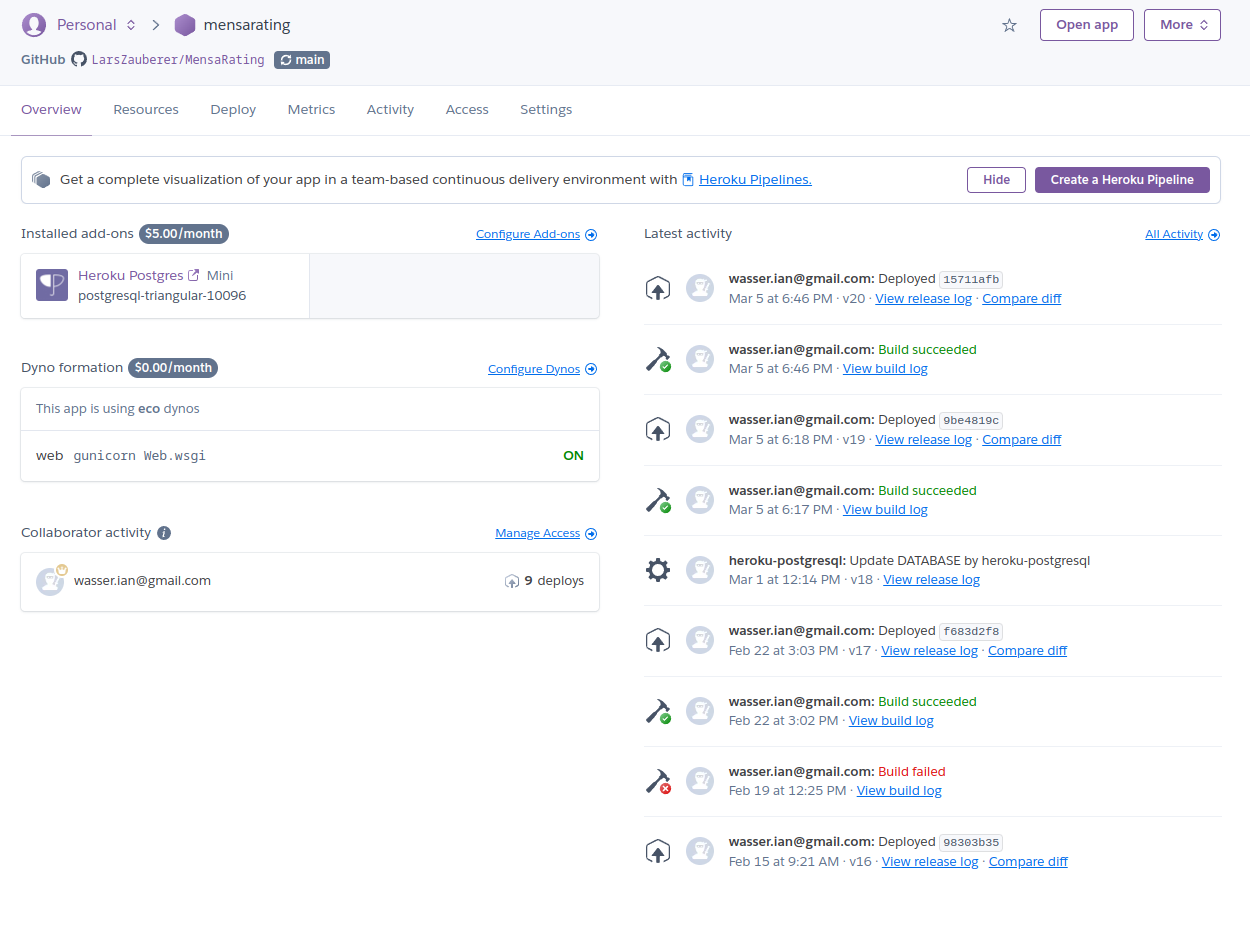
\includegraphics[width=0.8\textwidth]{images/Heroku.png}
    \caption{Screenshot: Heroku Interface für die App}
    \label{fig:r-deployment}
\end{figure}

Die Webseite wurde auf Heroku (siehe Interface der Heroku App
\ref{fig:r-deployment}) mit einem Eco-Server und einer Postgres Datenbank
veröffentlicht.

\newpage

\subsection{Datenbank}

\begin{figure}[ht]
    \centering
    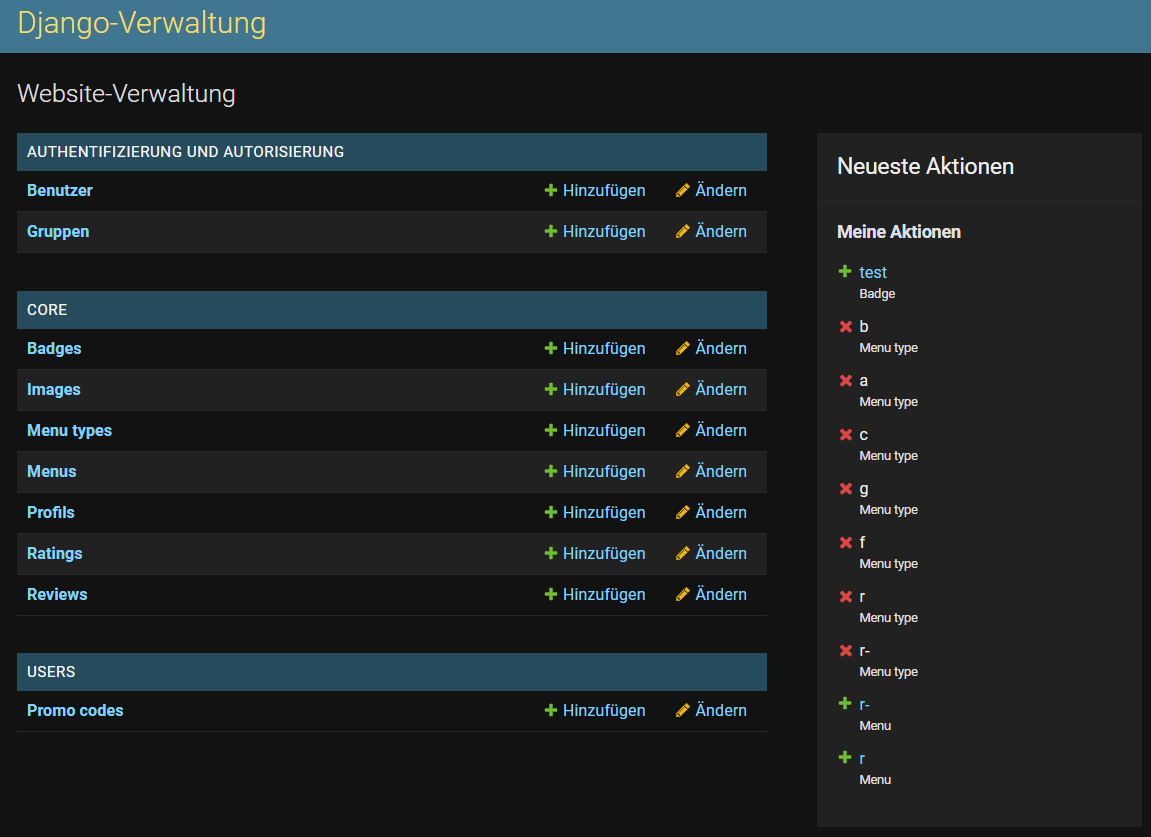
\includegraphics[width=0.8\textwidth]{images/Resultat-Adminpanel.png}
    \caption{Screenshot: Admin panel Web Page von Django}
    \label{fig:r-adminpanel}
\end{figure}

\begin{figure}[htp]
    \begin{subfigure}[b]{0.5\textwidth}
        \centering
        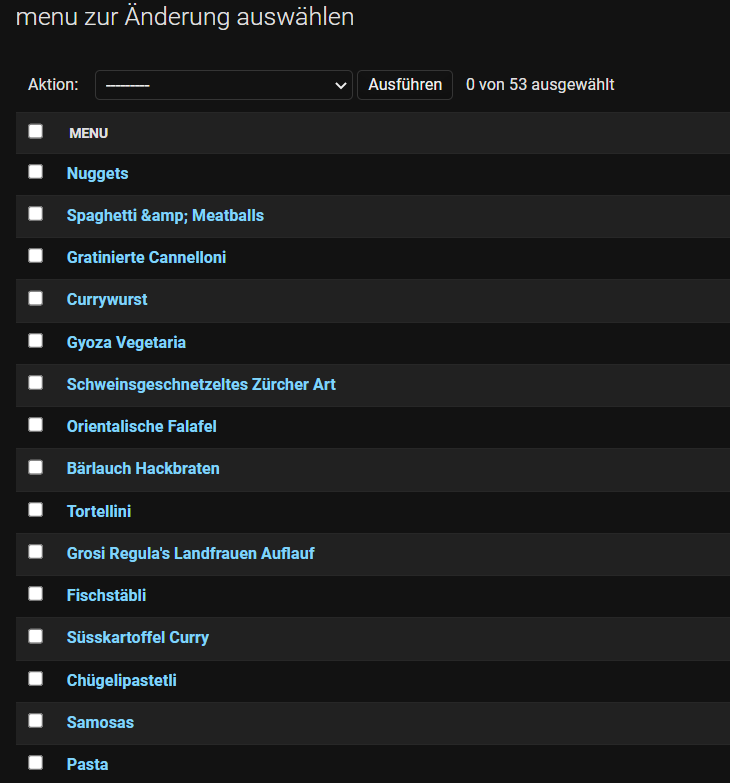
\includegraphics[width=0.7\textwidth]{images/Resultat-admin-menulist.png}
        \caption{Screenshot: Menu Einträge in Datenbank}
        \label{fig:r-adminpanel-menulist}
    \end{subfigure}
    \begin{subfigure}[b]{0.5\textwidth}
        \centering
        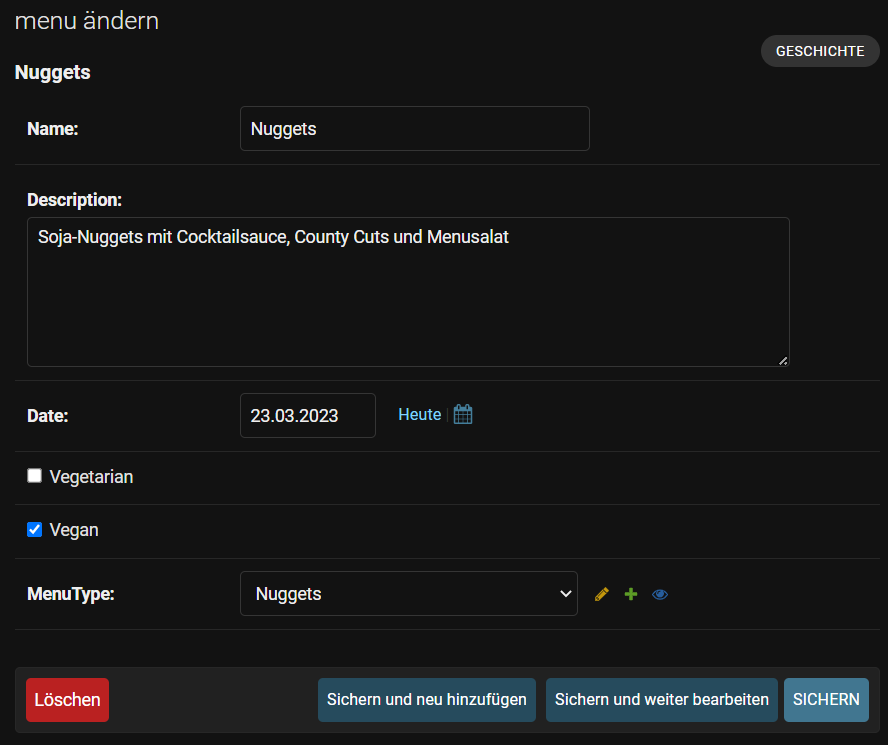
\includegraphics[width=0.7\textwidth]{images/Resultat-admin-menu.png}
        \caption{Screenshot: Spezifischer Menu Eintrag}
        \label{fig:r-adminpanel-menu}
    \end{subfigure}
    \hfill
    \begin{subfigure}[b]{\textwidth}
        \centering
        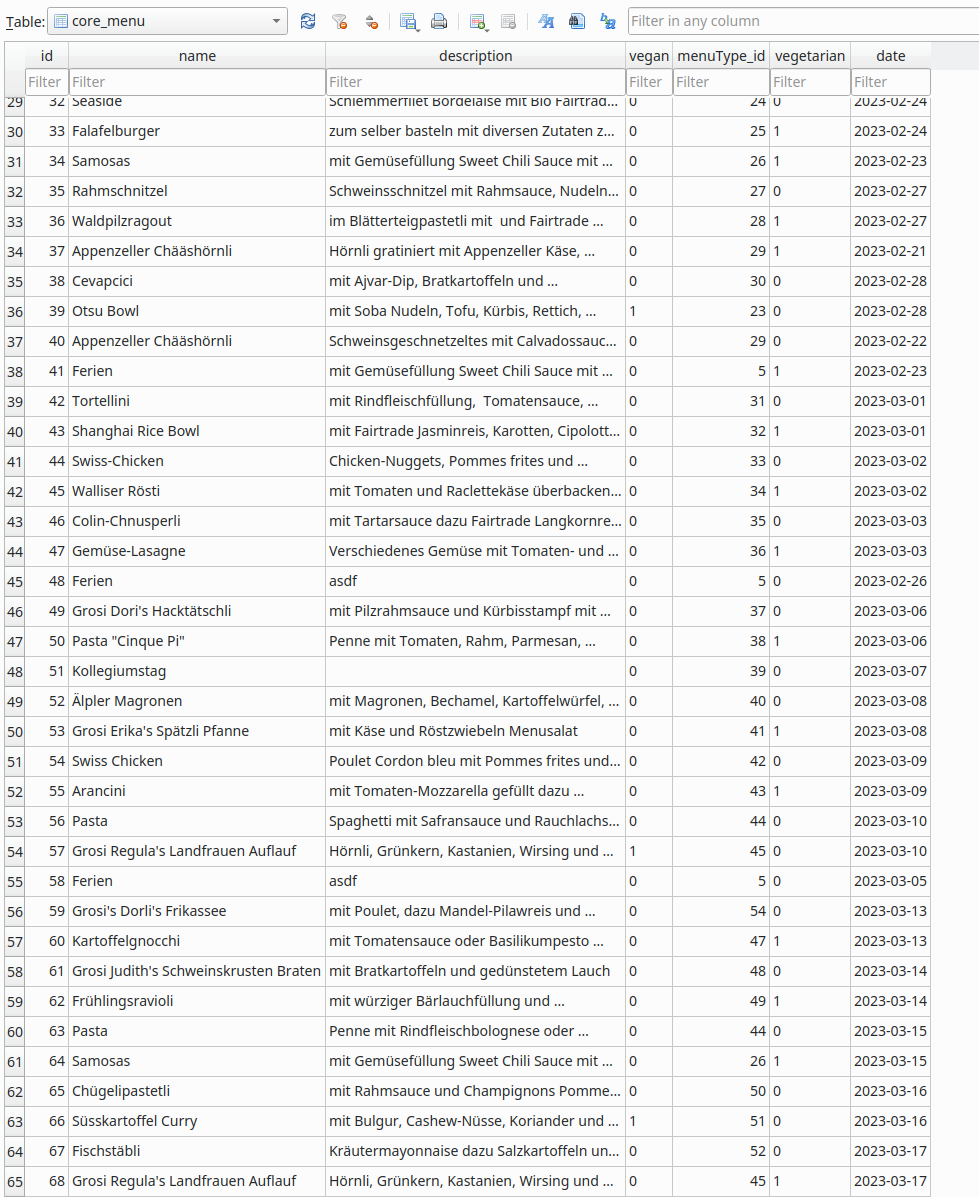
\includegraphics[width=\textwidth]{images/SQL.png}
        \caption{Screenshot: Menu Tabelle aus der rohen SQL-Datei}
        \label{fig:r-SQL-menu}
    \end{subfigure}
\end{figure}

\newpage
Auf dem bereitgestellten Admin Panel von Django (siehe \ref{fig:r-adminpanel})
können Administratoren Einträge in der Datenbank hinzufügen, löschen und
verändern.



\chapter{Diskussion und Ausblick}\label{chap:diskussion}

\section{Diskussion}\label{sub:diskussion}

Schlussendlich funktionieren alle Anforderungen und somit wurde das Projekt
realistisch geplant. Schwierigkeiten machte der Webscraper, da dieser Änderungen
auf der offiziellen Mensa Website erfassen und übernehmen musste.

\section{Ausblick}\label{sub:ausblick}

Folgende Erweiterungen der WebApp wären denkbar: 
\begin{itemize}
    \item Mehr Sortier- und Filter-Funktionen: z.B die Möglichkeit, aufsteigend
    oder absteigend zu sortieren.
    \item Subkommentare: Die Möglichkeit, auf ein Review eine Antwort in Form
    eines likebaren Kommentars geben zu können.
\end{itemize}





\chapter{Implementierung}
\section{core.models.py}\label{code:core.models.py}
\begin{lstlisting}[language=Python]
from django.db import models  # The django default model
from django.conf import settings  # To gain access to the settings of the app
from django.contrib.auth.models import User  # To gain access to the django internal user
from django.core.validators import MinValueValidator, MaxValueValidator  # For the Rating to validate if the rating is in the range of 1-5

import datetime as dt  # to handle dates

from django.core.files.storage import FileSystemStorage  # To get the default storage service from django

if settings.HEROKU:
    from gdstorage.storage import GoogleDriveStorage
    # Define Google Drive Storage
    storage_service = GoogleDriveStorage()
else:
    # Define normal MEDIA Storage Directory
    storage_service = FileSystemStorage()
    


class Profil(models.Model):
    """
    Profil class for the user. A custom class to add more information to the user.
    """
    karma = models.IntegerField(default=0)  # Karma points for the posts from the user. 
    user = models.OneToOneField(User, on_delete=models.CASCADE)  # User linked to the profil. -> The profil is deleted when the user is deleted.
    picture = models.ImageField(upload_to='profile_images', storage=storage_service, blank=True, null=True)  # Image of the user.

    def __str__(self):
        """
        __str__ Returns the username of the user owning the profil.

        :return: Returns the username of the user owning the profil.
        :rtype: str
        """
        return self.user.username


class MenuType(models.Model):
    """
    MenuType class for the type of the menu
    """
    name = models.CharField(max_length=100, unique=True)

    def __str__(self):
        """
        __str__ Returns the name of the mealtype.

        :return: Returns the name of the mealtype.
        :rtype: str
        """
        return self.name


class Menu(models.Model):
    """
    Menu class for the meals in the Mensa.
    """
    name = models.CharField(max_length=100)  # Name of the meal.
    description = models.TextField()  # Description of the meal.
    date = models.DateField(default=dt.date.today())  # Date of the meal. Default is the current date.
    vegetarian = models.BooleanField(default=False)  # Is the meal vegetarian?
    vegan = models.BooleanField(default=False)  # Is the meal vegan
    menuType = models.ForeignKey(MenuType, on_delete=models.CASCADE)

    def __str__(self):
        """
        __str__ Returns the name of the meal.

        :return: Returns the name of the meal.
        :rtype: str
        """
        return self.name


class Review(models.Model):
    """
    Review class for the reviews of the meals.
    """
    profil = models.ForeignKey(Profil, on_delete=models.SET_NULL, null=True)  # Profil of the user who wrote the review. -> If the user doesn't exist anymore, the review is still there.
    menu = models.ForeignKey(Menu, on_delete=models.CASCADE)  # Menu of the meal the review is about. -> If the meal doesn't exist anymore, the review is deleted.
    likes = models.IntegerField(default=0)  # Number of likes for the review.
    text = models.TextField(max_length=200) # Text of the review.


    date = models.DateTimeField(auto_now_add=True)  # Date of the review. Default is the current date.
    
    def __str__(self):
        """
        __str__ Returns the text of the review.

        :return: Returns the text of the review.
        :rtype: str
        """
        #return f"{self.profil.user.username}: {self.text[0:20]}..."
        return f"rew.{self.pk}"


class Image(models.Model):
    """
    Image class for the images of the meals.
    """

    profil = models.ForeignKey(Profil, on_delete=models.SET_NULL, null=True)  # Profil of the user who uploaded the image. -> If the user doesn't exist anymore, the image is still there.
    menu = models.ForeignKey(Menu, on_delete=models.CASCADE)  # Menu of the meal the image is about. -> If the meal doesn't exist anymore, the image is deleted.
    image = models.ImageField(upload_to='images/', storage=storage_service)  # Image of the meal.
    likes = models.IntegerField(default=0)  # Number of likes for the image.
    date = models.DateTimeField(auto_now_add=True)  # Date of the image. Default is the current date.
    
    def __str__(self):
        """
        __str__ Returns the name of the image.

        :return: Returns the name of the image.
        :rtype: str
        """
        if self.profil:
            return f"{self.profil.user.username}: {self.image.name}"
        else:
            return f"None: {self.image.name}"


class Rating(models.Model):
    profil = models.ForeignKey(Profil, on_delete=models.SET_NULL, null=True)  # Profil of the user who rated the meal. -> If the user doesn't exist anymore, the rating is still there.
    menu = models.ForeignKey(Menu, on_delete=models.CASCADE)  # Menu of the meal the rating is about. -> If the meal doesn't exist anymore, the rating is deleted.
    rating = models.IntegerField(validators=[MinValueValidator(1), MaxValueValidator(5)], default=1)  # Rating of the meal.


class Badge(models.Model):
    name = models.CharField(max_length=50)
    description = models.TextField()
    image = models.ImageField(upload_to="images/", storage=storage_service)

    condition_category = models.IntegerField()
    count = models.IntegerField()
    
    def __str__(self):
        return self.name

\end{lstlisting}
\section{core.webscraper.py}\label{code:core.webscraper.py}
\begin{lstlisting}[language=Python]
# https://www.crummy.com/software/BeautifulSoup/bs4/doc/

from bs4 import BeautifulSoup
import requests
import re
from .models import Menu, MenuType
import logging
import datetime as dt

log = logging.getLogger("Webscraper")

def get_menu_list(days):
    menuListDict = {}

    for menuIndex, day in enumerate(days):
        dishesOfDayDict = {}
        dishes = day.find_all(attrs={"class":"menu-item"})
        
        for dishIndex, dish in enumerate(dishes):
            dishDict = {}

            # get title and description of dish with html tags as strings and using the "clean()" function to remove tags and double spaces
            title = clean(str(dish.find("h2")))
            description = clean(str(dish.find(attrs={"class":"menu-description"})))
            
            # find out if dish is served with meat (0), vegetarian (1) or vegan (2)
            if (dish.find(attrs={"class":"label label-vegetarian has-infobox"}) is not None):
                label = 1
            elif (dish.find(attrs={"class":"label label-vegan has-infobox"}) is not None):
                label = 2
            else:
                label = 0

            # add gathered information to current dish of the day in the list
            dishDict["title"] = title
            dishDict["description"] = description
            dishDict["label"] = label
            
            # add complete menu to the list
            dishesOfDayDict[f"dish{dishIndex}"] = dishDict

        
        # add all menus of the day to the list
        menuListDict[f"menu{menuIndex}"] = dishesOfDayDict
    
    # return list of every menu of every day
    return menuListDict

def clean(str):
    # uses regex to substitute tags and double spaces in messy html string with empty strings or single spaces
    string = re.sub('<p class="menu-description">|</p>|<h2 class="menu-title">|</h2>|\\xad\s*|\\n', '', str)
    string = string.replace("<br/>", " ")
    return string

def get_day_data():
    page = requests.get("https://neuekanti.sv-restaurant.ch/de/menuplan/")
    soup = BeautifulSoup(page.content, "html.parser")
    return soup.find_all(attrs={"class":"menu-plan-grid"})

def get_dates():
    page = requests.get("https://neuekanti.sv-restaurant.ch/de/menuplan/")
    soup = BeautifulSoup(page.content, "html.parser")
    day_nav = soup.find_all(attrs={"class": "day-nav"})[0]
    dates = day_nav.find_all(attrs={"class": "date"})
    
    for i, el in enumerate(dates):
        date = dt.datetime.strptime(el.contents[0], "%d.%m.").date()
        date_td = dt.date.today()
        date = date.replace(year=date_td.year)
        # check if this date is already happend -> Can happen at the end of the year
        if date < date_td:
            date = date.replace(year=date_td.year + 1) # set it to next year
        dates[i] = date
    
    return dates

def main():
    days = get_day_data()
    get_dates()
    
    # Print
    for dishesOfDay in get_menu_list(days).values():
        for dish in dishesOfDay.values():
            for element in dish.values():
                print(element)
            print("")
    
    print(get_menu_list(days))

def webscrape():
    days = get_day_data()  # Get all the days
    dates = get_dates()  # Get the dates of the days
    return get_menu_list(days), dates  # Retrive all the information

def create_menu_in_database(title, description, label, date):
    menuType = MenuType.objects.filter(name=title)
    if len(menuType) == 0:
        log.info(f"No menuType with the name: {title} found.")
        menuType = [MenuType.objects.create(name=title)]
        log.info(f"Created menuType: {menuType[0]}")
    menuType = menuType[0]
    
    labels = [
        {"vegetarian": False, "vegan": False},
        {"vegetarian": True, "vegan": False},
        {"vegetarian": False, "vegan": True},
    ]
    
    Menu.objects.create(name=title, description=description, menuType=menuType, date=date, **labels[label])
    

def sync_today_menu():
    log.debug(f"Retrieving mensa data")
    data, dates = webscrape()
    log.debug(f"Data received: {data}, {dates}")

    for key, date in zip(data.keys(), dates):
        # Check if todays menu is already in database
        log.debug(f"Checking if menu of date ({date}) is already in the database")
        menus = Menu.objects.filter(date=date)
        
        # Compare database with the data from the website
        titles = [i.name for i in menus]
        for i in data[key].keys():
            if data[key][i]["title"] not in titles:
                # Menu not in the database
                log.info(f"Menu \"{data[key][i]['title']}\" is not in the database")
                create_menu_in_database(data[key][i]["title"], data[key][i]["description"], data[key][i]["label"], date)  # Create the menu
                log.info(f"Created menu: {data[key][i]['title']}")
            else:
                log.debug(f"Menu \"{data[key][i]['title']}\" already in database")


if __name__ == "__main__":
    main()
\end{lstlisting}
\section{core.views.py}\label{code:core.views.py}
\begin{lstlisting}[language=Python]
# Maintained by: Robin, Ian
# pylint: disable=no-member
from django.http import HttpResponse  # To send a simple response to the user
from django.contrib import messages  # To send alert messages to the user
from datetime import datetime as dt  # for date and time
import logging  # To gain logging information
from django.shortcuts import render, redirect  # To render the html page and redirect to another page
from django.urls import reverse  # To get the url of a page
import datetime as dt  # for date and time
from .models import MenuType, Menu, Review, Image, Profil  # To gain access to the database
from .statistic_functions import *  # To gain access to the statistic functions
from .forms import ImageForm, ReviewForm, RatingForm, ProfilPictureForm  # Create user forms
from .post_functions import postImage, postRating, postReview  # To gain access to the post functions
from .webscraper import sync_today_menu  # To gain access to the webscraper


def index(request):
    sync_today_menu()

    # Get all menus with the date today
    menus = Menu.objects.filter(date__gte=dt.date.today(), date__lte=dt.date.today() + dt.timedelta(days=7)).order_by("date")  # gte = greater than or equal
    
    dates = []
    menus_with_date = []
    for i, menu in enumerate(menus):
        # Check if the date, when a menu occured is already listed 
        if menu.date not in dates:
            dates.append(menu.date)
            menus_with_date.append([])
        
        # Get best image of the menu
        img = get_all_images_sorted(menu.menuType)
        if img != None:
            img = img[0]
        
        # Add the menu to the list with all the informations
        menus_with_date[-1].append( (i, menu, img, getRating(menu), getNumRates(menu)) )
    menus = Menu.objects.filter(date=dt.date.today())

    # Calculate the rating for each menu
    ratings = [getRating(i) for i in menus]
    numRates = [getNumRates(i) for i in menus]

    # Get the highest rated image for each menu
    images = []
    for i in menus:
        img = get_all_images_sorted(i.menuType)
        if img != None:  # There is no highest image -> None
            images.append(img[0])
        else:
            images.append(None)


    # Zip the data together
    menus = zip(dates, menus_with_date)

    context = {'menus_dates': list(menus)}

    return render(request, 'index.html', context=context)


def menu(request, pk):
    sync_today_menu()
    log = logging.getLogger("menu")
    
    # Get the menu data
    menu = Menu.objects.filter(pk=pk)
    if len(menu) == 0:
        log.warning(f"Menu with pk:{pk} not found")
        return HttpResponse("Menu not found")
    menu = menu[0]
    
    today = menu.date == dt.date.today() # Save if the menu is a menu of today
    
    # Check if the request is a post request
    if request.method == "POST" and today:
        log.debug(f"Post Data received: {request.POST}")
        log.debug(f"Files received: {request.FILES}")
        form = None

        # Sort different post kinds
        # Rating
        if request.POST.get("rating"):
            form = RatingForm(request.POST)
            log.debug(f"Rating Form Recognized")
            msg = postRating(request, pk, form)

        # Review
        elif request.POST.get("text"):
            form = ReviewForm(request.POST)
            log.debug(f"Review Form Recognized")
            msg = postReview(request, pk, form)
        
        # Image
        elif request.FILES.get("image"):
            form = ImageForm(request.POST, request.FILES)
            log.debug(f"Image Form Recognized")
            msg = postImage(request, pk, form)
        
        # None of the valid kinds
        if form is None:
            log.warning(f"Form type is invalid for post data: {request.POST}")
            msg = ("Invalid Form Type", 1)
        
        # Return user alert message
        if msg[1] == 1:
            messages.error(request, msg[0])
        else:
            messages.success(request, msg[0])

    # Get the reviews
    reviews = Review.objects.filter(menu=menu).order_by("-likes")
    review_badges = []
    for i in reviews:
        if i.profil:
            review_badges.append(get_badges_of_profil(i.profil))
        else:
            review_badges.append([])

    # Get the images
    images = Image.objects.filter(menu=menu).order_by("-likes")
    image_badges = []
    for i in images:
        if i.profil:
            image_badges.append(get_badges_of_profil(i.profil))
        else:
            image_badges.append([])
    
    reviews = list(zip(reviews, review_badges))
    images = list(zip(images, image_badges))

    # Get the rating
    rating = getRating(menu)
    numRates = getNumRates(menu)
    

    # Forms
    imageForm = ImageForm()
    reviewForm = ReviewForm()
    ratingForm = RatingForm()

    context = {"menu": menu, "reviews": reviews, "images": images, "rating": rating, "numRates": numRates,
                "imageForm": imageForm, "reviewForm": reviewForm,
                "ratingForm": ratingForm, "today": today}  # Create a context dictionary to pass to the template

    return render(request, "menu.html", context=context)

def menuType(request, pk):
    sync_today_menu()
    log = logging.getLogger("menuType")
    
    menutype = MenuType.objects.filter(pk=pk)
    if len(menutype) == 0:
        log.warning(f"Menutype with pk:{pk} not found")
        return HttpResponse("Menutype not found")
    menutype = menutype[0]

    menu_instances = Menu.objects.filter(name=menutype.name).filter(date__lte=dt.date.today()).order_by("-date")
    

    # Set variables
    description = menu_instances[0].description
    vegetarian = menu_instances[0].vegetarian
    vegan = menu_instances[0].vegan

    
    # Calculate statistics
    occurrences = menu_instances.count()
    allTimeRating = getRatingOfAllTime(menutype)
    allTimeNumRates = getNumRatesOfAllTime(menutype)


    # Get the ratings
    ratings = [getRating(i) for i in menu_instances]
    numRates = [getNumRates(i) for i in menu_instances]
    indexes = list(range(len(menu_instances)))

    # Get the images for the menu type
    images = get_all_images_sorted(menutype)
    if images == None: images = []
    
    # Get the badges for the images
    image_badges = []
    for i in images:
        if i.profil:
            image_badges.append(get_badges_of_profil(i.profil))
        else:
            image_badges.append([])
    images = list(zip(images, image_badges))

    # Zip the data together
    menu_instances = zip(indexes[:600], ratings[:600], numRates[:600], menu_instances[:600])

    context = {"name": menutype.name, "description": description, "images": images, "vegetarian": vegetarian, "vegan": vegan, "menu_instances": menu_instances, "occurrences": occurrences, "allTimeRating": allTimeRating, "allTimeNumRates": allTimeNumRates}

    return render(request, "menuType.html", context=context)




def allMenu(request):
    sync_today_menu()
    
    menuTypes = MenuType.objects.all()
    
    # lists with all the datas
    occurrences = []
    allTimeRatings = []
    allTimeNumRates = []
    descriptions = []
    vegetarians = []
    vegans = []

    # Get all the data and save it in the lists
    for typ in menuTypes:
        menus = Menu.objects.filter(name=typ.name).filter(date__lte=dt.date.today())
        if len(menus) > 0:
            descriptions.append(menus[0].description)
            vegetarians.append(menus[0].vegetarian)
            vegans.append(menus[0].vegan)
            occurrences.append(menus.count())
            allTimeRatings.append(getRatingOfAllTime(typ))
            allTimeNumRates.append(getNumRatesOfAllTime(typ))
        
    indexes = list(range(len(menuTypes))) 

    # Zip the informations together
    menuType_info = zip(indexes, menuTypes, occurrences, descriptions, vegetarians, vegans, allTimeRatings, allTimeNumRates)


    #Order by number of occurrences
    #menuType_info = sorted(menuType_info, key=lambda x: x[2], reverse=True)  # Sort the menu info after occurrences -> lowest to highest

    context = {"menuTypes": menuType_info}


    
   

    return render(request, "allMenu.html", context=context)


def timeline(request):
    sync_today_menu()
    menus = Menu.objects.filter(date__lte=dt.date.today()).order_by("-date")
    
    dates = []
    menus_with_date = []
    for i, menu in enumerate(menus):
        # Check if the date, when a menu occured is already listed 
        if menu.date not in dates:
            dates.append(menu.date)
            menus_with_date.append([])
        
        # Add the menu to the list with all the informations
        menus_with_date[-1].append( (i, menu, getRating(menu), getNumRates(menu)) )

    # Zip the dates and the menus together. Show only 600
    menu_dates = zip(dates[:600], menus_with_date[:600]) # Return the first 600 menus


    context = {"menu_dates": menu_dates}  


    return render(request, "timeline.html", context=context)


def userProfile(request):
    sync_today_menu()
    
    # Check if the user is logged in -> If not redirect to login page
    if not request.user.is_authenticated:
        return redirect(reverse("login"))
    
    # Get the profil
    profil = Profil.objects.get(user=request.user)
    
    # Calculate all the badges. And calculate what the user has or has not achieved.
    # Uploading a new profil picture
    if request.method == "POST":
        form = ProfilPictureForm(request.POST, request.FILES)
        if form.is_valid():
            img = form.instance.picture
            profil.picture = img
            profil.save()
    
    badges = get_badges_of_profil(profil)
    all_badges = []
    for i in range(3): # 3 Badge categories
        all_badges.append(list(Badge.objects.filter(condition_category=i).order_by("count")))
        
    for i in all_badges:
        for e, el in enumerate(i):
            i[e] = (el, el in badges)  # Tag all the badges the profil posses
    
    # Get the reviews and images of the profil
    reviews = Review.objects.filter(profil=profil).order_by("-likes")
    images = Image.objects.filter(profil=profil).order_by("-likes")
    
    # Image uploading form
    imageForm = ProfilPictureForm()

    context = {"name": profil.user, "karma": profil.karma, "badges": all_badges, "images": images, "reviews": reviews, "imageForm": imageForm, "picture": profil.picture}

    return render(request, "userProfile.html", context=context)


def like(request, cat: int, pk: int):
    log = logging.getLogger("Like View")
    
    # All models that can be liked
    obj_cat: dict = {
        1: Review,
        2: Image
    }
    
    obj = obj_cat.get(cat)
    
    # Is the category index out of range for the dict
    if not obj:
        log.warning(f"Category: {cat} out of range")
        return HttpResponse("Category not found")
    
    log.debug(f"Model recognized: {obj}")
    
    post = obj.objects.filter(pk=pk)  # Get the post object from the database
    
    # If a post found
    if len(post) == 0:
        log.warning(f"No model of type {obj} with pk {pk} found!")
        return HttpResponse("Post not found")

    post = post[0]
    
    # Check if the post is from today
    if post.menu.date != dt.date.today():
        log.warning(f"Post is to old")
        return HttpResponse("Post cannot be liked anymore")
    
    # Check if dislike or like
    dislike = request.GET.get("dislike")
    
    # Check if this should be a dislike
    weight = 1
    if dislike:
        log.debug(f"Dislike: {dislike}")
        weight = -1
    
    # Like the post
    post.likes += weight
    
    # If the like count is below zero -> 0
    if post.likes < 0:
        post.likes = 0
        
    if post.profil is not None:
        post.profil.karma += weight
        post.profil.save()
    
    post.save()  # Save to the database
    
    return HttpResponse(post.likes)


def leaderboard(request):
    sync_today_menu()
    
    profils = Profil.objects.all().order_by("-karma")
    
    user_profil = None
    rang = None
    if request.user.is_authenticated:
        user_profil = Profil.objects.get(user=request.user)
        rang = list(profils).index(user_profil) + 1
        
    profils = profils[:20]
    badges = []
    for i in profils:
        badges.append(get_badges_of_profil(i))
    
    context = {"profils": zip(profils, badges), "user_profil": user_profil, "rang": rang}
    
    return render(request, "leaderboard.html", context=context)

\end{lstlisting}
\section{core.urls.py}\label{code:core.urls.py}
\begin{lstlisting}[language=Python]
from .views import *
from django.urls import path
from django.conf import settings
from django.conf.urls.static import static

urlpatterns = [
    path('menu/<int:pk>', menu, name="menu"),
    path('allMenu', allMenu, name="allMenu"),
    path('userProfile', userProfile, name="userProfile"),
    path('menuType/<int:pk>', menuType, name="menuType"),
    path('timeline', timeline, name="timeline"),
    path('like/<int:cat>/<int:pk>', like, name="like"),
    path('leaderboard', leaderboard, name="leaderboard"),
    path('', index, name="index"),
]

if settings.DEBUG:  # new
    urlpatterns += static(settings.MEDIA_URL, document_root=settings.MEDIA_ROOT)
    urlpatterns += static(settings.STATIC_URL, document_root=settings.STATIC_ROOT)
    
\end{lstlisting}
\section{core.statistic-functions.py}\label{code:core.statistic-functions.py}
\begin{lstlisting}[language=Python]
# Maintained by: Robin, Ian

from .models import MenuType, Menu, Rating, Image, Profil, Badge, Review  # To have access to the database
from django.db.models import Avg, Max  # To use statistic functions of the database
import logging  # To gain logging information

log = logging.getLogger("statistic_functions")

def getRating(menu):
    # Get the ratings
    rating = Rating.objects.filter(menu=menu).aggregate(Avg("rating"))

    if rating["rating__avg"] == None:
        return 0
    else:
        return float('%.1f' % rating["rating__avg"])


def getRatingOfAllTime(menuType):
    # Find all menu occurencies
    menus = Menu.objects.filter(menuType=menuType)

    # Find all ratings for all the menu occurencies
    rating = Rating.objects.filter(menu__in=menus).aggregate(Avg("rating"))

    if rating["rating__avg"] == None:
        return 0
    else:
        return float('%.1f' % rating["rating__avg"])


def get_all_images_sorted(menuType):
    allmenus = Menu.objects.filter(menuType=menuType)
    images = Image.objects.filter(menu__in=allmenus).order_by("-likes")

    if len(images) == 0:
        return None
    else:
        return images


def get_all_reviews_sorted(menuType):
    allmenus = Menu.objects.filter(menuType=menuType)
        
    reviews = Review.objects.filter(menu__in=allmenus).order_by("-likes")

    if len(reviews) == 0:
        return None
    else:
        return reviews

def count_best_posts_of_profil(profil: Profil, best_post_function) -> int:
    # Count of most liked images
    menuTypes: list[MenuType] = MenuType.objects.all()
    counter: int = 0
    for i in menuTypes:
        if  best_post_function(i) != None:
            post = best_post_function(i)[0]
            if post.profil == profil:
                counter += 1
    
    return counter

def getNumRates(menu):
    return Rating.objects.filter(menu=menu).count()
    
def getNumRatesOfAllTime(menuType):
    menus = Menu.objects.filter(menuType=menuType)
    return Rating.objects.filter(menu__in=menus).count()

def get_badges_of_profil(profil: Profil):
    karma: int = profil.karma

    badges: list[Badge] = Badge.objects.all()
    
    img_counter: int = count_best_posts_of_profil(profil=profil, best_post_function=get_all_images_sorted)
    review_counter: int = count_best_posts_of_profil(profil=profil, best_post_function=get_all_reviews_sorted)
    categories: list[int] = [karma, img_counter, review_counter]
    
    # Get the highest badge for all the categories
    highest_badges: list[Badge] = [None for _ in categories]
    for i in badges:
        if i.count <= categories[i.condition_category]:  # Does the profil have this badge
            # Check if the badge is more worth than the saved.
            if highest_badges[i.condition_category] is None:
                highest_badges[i.condition_category] = i
            else:
                if highest_badges[i.condition_category].count < i.count:
                    highest_badges[i.condition_category] = i
    
    highest_badges = [i for i in highest_badges if i is not None]  # Remove all None
    
    return highest_badges

\end{lstlisting}
\section{static.js.allmenu-statistics.js}\label{code:static.js.allmenu-statistics.js}
\begin{lstlisting}
//Maintained by Robin, Valentin
//This File handles the filter/sorting of the menutypes on the allMenu.html page

//different order options. Data gets saved in menuTypes array
function orderMenutypes(orderType) {
    if (orderType == "occ") {
        menuTypes.sort(function (a, b) {
            let x = a.occurrences;
            let y = b.occurrences;
            //descending order
            if (x < y) return 1;
            else if (x > y) return -1;
            return 0;
        })
    }
    else if (orderType == "rating") {
        menuTypes.sort(function (a, b) {
            let x = a.rating;
            let y = b.rating;
            //descending order
            if (x < y) return 1;
            else if (x > y) return -1;
            return 0;
        })
    }
    else if (orderType == "numrates") {
        menuTypes.sort(function (a, b) {
            let x = parseInt(a.numrates);
            let y = parseInt(b.numrates);
            //descending order
            if (x < y) return 1;
            else if (x > y) return -1;
            return 0;
        })
    }
    else if (orderType == "name") {
        menuTypes.sort(function (a, b) {
            return a.name.localeCompare(b.name); // alphabetical order
        })
    }
    updateListboxs()
    toggleStatOptions(1)
}

//different filter options. Data gets saved in menuTypes array
function filterMenutypes(filterType) {
    for (let i = 0; i < menuTypes.length; i++) {
        let menuType = menuTypes[i]
        //set visibility attribute of each menuType according to filter
        if (filterType == "vegan") {
            if (menuType.vegan == "True") menuType.visible = true;
            else menuType.visible = false;
        } else if (filterType == "vegi") {
            if (menuType.vegetarian == "True") menuType.visible = true;
            else menuType.visible = false
        }
        else {
            menuTypes[i].visible = true
        }
    }
    //update menus according to options
    updateListboxs()
    toggleStatOptions(0)
}

//update the html of the listboxes with the sorted/filter data in the menuTypes array
function updateListboxs() {
    for (let i = 0; i < menuTypes.length; i++) {
        let menuTypeObject = document.getElementById("menutype-" + i);
        let menuType = menuTypes[i]

        //make menutypes width visible == false invisible
        menuTypeObject.style.display = "flex"
        if (!menuType.visible) {
            menuTypeObject.style.display = "None"
        }
        else {
            menuTypeObject.setAttribute("onclick", "location.href='" + menuType.url + "';") //assign correct link to menu
            menuTypeObject = menuTypeObject.children
            menuTypeObject[0].innerHTML = menuType.name //first div == name
            
            let vegivegan = menuTypeObject[1].children;

            if (menuType.vegetarian == "True") {
                vegivegan[0].style.display = "block"; //show vegetarian label
            } else if (menuType.vegan == "True") {
                vegivegan[1].style.display = "block"; //show vegan label
            }

            menuTypeObject[2].innerHTML = "Vorkommen: " + menuType.occurrences //show occurrences

            //update Rating
            rating = menuTypeObject[3].children
            rating[0].innerHTML = menuType.rating
            starRate(i, menuType.rating)
            rating[2].innerHTML = "(" + menuType.numrates + ")"
        }
    }
}

//Toggles visibility of the Options for filter/sorting
//Argument type (int): 0 -> targets filter button, 1 -> targets sort button
function toggleStatOptions(type) {
    let orderoptions = document.getElementsByClassName("stat-criteria")[type]
    let orderButtons = orderoptions.children

    if (orderoptions.style.height == "" || orderoptions.style.height == "0em") { //if not visible
        orderoptions.style.height = "1em"
        for (let i = 0; i < orderButtons.length; i++) { //Make every option visible
            orderButtons[i].style.height = "2em"
            orderButtons[i].style.opacity = 1;
        }
    }
    else { //currently visible
        orderoptions.style.height = "0em"
        for (let i = 0; i < orderButtons.length; i++) { //make every option invisible
            orderButtons[i].style.height = "0em"
            orderButtons[i].style.opacity = 0
        }
    }
}
\end{lstlisting}



%% Your Appendix
\appendix

\backmatter

% \bibliographystyle{plain}
% \bibliography{refs}

\printbibliography[heading=bibintoc]

\begin{KeepFromToc}
\listoffigures
\end{KeepFromToc}

\end{document}
